\documentclass[11pt,a4paper]{article}
\usepackage[margin=22mm,headheight=16pt]{geometry}
\usepackage{fontspec}
\setmainfont[Path=../fonts/,BoldFont=NotoSerifCJKsc-Bold.otf,ItalicFont=NotoSerifCJKsc-Regular.otf]{NotoSerifCJKsc-Regular.otf}
\setsansfont[Path=../fonts/,BoldFont=NotoSerifCJKsc-Bold.otf]{NotoSerifCJKsc-Regular.otf}
\setmonofont{DejaVu Sans Mono}
\XeTeXlinebreaklocale "zh"
\XeTeXlinebreakskip=0pt plus 1pt
\usepackage{amsmath,amssymb,amsthm,mathtools}
\usepackage{graphicx,booktabs,longtable,array,enumitem,xcolor}
\usepackage{hyperref,fancyhdr,caption,needspace}
\hypersetup{colorlinks=true,linkcolor=blue!45!black,citecolor=blue!45!black,urlcolor=blue!55!black,pdftitle={Research W: 未知复杂墙体的 Maxwell 传播可辨识性与概率成像},pdfauthor={Research W}}
\urlstyle{same}
\setlength{\parindent}{0pt}
\setlength{\parskip}{5pt}
\linespread{1.13}
\setlength{\emergencystretch}{4em}
\setcounter{tocdepth}{2}
\setlist{nosep,leftmargin=1.8em,topsep=4pt}
\renewcommand{\contentsname}{目录}
\renewcommand{\refname}{参考文献与固定版本研究来源}
\renewcommand{\figurename}{图}
\renewcommand{\tablename}{表}
\newtheorem{proposition}{命题}[section]
\newtheorem{theorem}[proposition]{定理}
\newtheorem{lemma}[proposition]{引理}
\newtheorem{corollary}[proposition]{推论}
\theoremstyle{definition}
\newtheorem{definition}[proposition]{定义}
\newtheorem{example}[proposition]{反例}
\theoremstyle{remark}
\newtheorem*{remark}{适用边界}
\renewcommand{\proofname}{证明}
\newcommand{\E}{\mathbb E}
\newcommand{\Prob}{\mathbb P}
\newcommand{\R}{\mathbb R}
\newcommand{\C}{\mathbb C}
\newcommand{\TV}{\operatorname{TV}}
\newcommand{\range}{\operatorname{Range}}
\newcommand{\diag}{\operatorname{diag}}
\newcommand{\supp}{\operatorname{supp}}
\newcommand{\KL}{\operatorname{KL}}
\newcommand{\tr}{\operatorname{tr}}
\newcommand{\argmin}{\operatorname*{arg\,min}}
\newcommand{\argmax}{\operatorname*{arg\,max}}
\pagestyle{fancy}
\fancyhf{}
\fancyhead[L]{\small Research W}
\fancyhead[R]{\small 未知环境 · 传播可辨识性 · 概率成像}
\fancyfoot[C]{\small \thepage}
\begin{document}
\begin{titlepage}
\vspace*{18mm}
{\LARGE\bfseries Research W\par}
\vspace{8mm}
{\huge\bfseries 未知复杂墙体的 Maxwell\\[3mm]传播可辨识性与概率成像\par}
\vspace{7mm}
{\Large 从联合材料歧义到任务相关传播学习\par}
\vspace{10mm}
{\large Self-Calibrating Maxwell Imaging Through Unknown\\Heterogeneous and Irregular Walls\par}
\vspace{15mm}
\begin{quote}
\textbf{本报告的中心判断}\\[3pt]
值得开展一个范围明确的独立理论分支，但应先回答“已有观测能否确定下游任务所需的传播”，再决定是否设计递进算法。按深度更新 Green 不是新的信息来源；不确定环境的任务传播风险及其可计算界，才是最值得检验的科学对象。
\end{quote}
\vfill
研究对象：有限单侧孔径、有限带宽、未知总材料场与 nuisance\\
交付性质：中文理论报告、来源审计、已执行的一维解析核验、P0/P1 实验协议\\
证据截止：2026 年 10 月 22 日\\
本轮没有执行二维或三维成像实验、训练网络或建立完整后验参考。
\end{titlepage}
\tableofcontents
\clearpage
\section{执行判断与证据分级}
\subsection{建议保留什么，先停止什么}
Research W 的独立价值不在于把“成像、更新背景、再成像”重新组合。DBIM 已在不均匀当前背景上反复线性化；layer stripping 与 invariant embedding 已研究边界响应的向内推进；Marchenko/redatuming 已研究从单侧反射恢复内部 Green 响应；Bayesian 与 goal-oriented inversion 已把参数不确定性传递到任务量。\cite{L_DBIM,L_Somersalo,L_EM2017,L_Marchenko22,L_Goal}

更值得立项的问题是：
\begin{quote}
在明确的单侧采集、合法材料类、目标任务类和噪声水平下，哪些观测无法区分的环境，会产生不同的完整目标响应？能否识别并保留这些传播分支，同时证明哪些分支可以安全合并？
\end{quote}

这是把关注点从“墙体材料是否重建正确”转移到“对指定成像任务，环境还存在哪些不可消除的传播歧义”。两者可能分离：材料不唯一而任务可辨识，也可能墙体回波拟合很好而目标传播不可靠。

\textbf{首选路线：传播可辨识性与不可能性。} 首轮以普通非磁、被动材料的有限非线性见证、联合目标补偿和任务误差下界为主。概率传播压缩作为其建设性后续；A17 是可选计算接口。不要先训练 Flow/Diffusion，也不要先搭建完整“逐层智能成像系统”。

\subsection{本轮实质结果}
本报告给出如下可检查成果，而非宣称已解决任意复杂墙体成像。
\begin{enumerate}
\item 明确总材料场与“墙/目标”语义分解的区别，给出无结构约束时的标签重分配自由度。
\item 给出任务可辨识的精确纤维判据、局部条件、有限维稳定常数及无限维反例；把目标和仪器补偿纳入局部观测算子。
\item 构造非磁、无损介质墙的精确单频 Maxwell 反例：两墙反射相同，双程目标响应不同；允许目标位移后，完整联合数据又完全相同。
\item 提出应保留的四块传播签名，覆盖背景响应、入射、接收及目标域内部反馈；推导远离共振时的响应误差界。
\item 证明在原联合先验不变的条件下，传播近似如何通过 likelihood 误差控制目标后验误差；指出仅聚类墙体后验不足以保留目标条件分布。
\item 用随机 Schur 响应定义可回退的计算前沿，并说明它通常不是按深度嵌套的物理层。
\item 核验 A17 最新 closure 与效率 follow-up，修正“只有冻结 GN、没有非线性后果”的过时总结；同时保留 A26、A30、F3、P2 的负结果。
\item 实际运行一维精确传输矩阵核验和带宽扫描，附完整代码与原始结果。二维复杂墙体的关键实验尚待执行。
\end{enumerate}

\Needspace{14\baselineskip}
\subsection{数学成立与论文原创性必须分开}
下文采用五类状态。
\begin{longtable}{p{27mm}p{121mm}}
\toprule
状态 & 含义\\
\midrule
已知工具 & resolvent、Schur、Woodbury、T-matrix、条件概率、二点检验与标准伴随残差恒等式。\\
本次可证推论 & 在正文明确假设下给出证明，但尚未建立文献首创性。四块签名稳定界、联合测度不变的压缩界属于此类。\\
解析反例 & 由完整 Maxwell 的严格子问题构造，已数值核对符号与参考平面；适用范围不能外推。\\
待检验机制 & 风险调度、传播分支搜索、可回退前沿及 A17 条件选空间的实际收益。\\
未解决 & 一般未知拓扑墙体的稳定全域后验、可靠跨拓扑混合、同成本算法优势和实际建筑穿透保证。\\
\bottomrule
\end{longtable}

一般的“反射不决定透射”在多模逆散射中已有明确讨论；本报告不会把这一概念、简单共振板反例或通用概率不等式冒称原创 Maxwell 定理。\cite{L_Waagaard} 强 IEEE TAP 贡献仍需把它收紧到可实现材料、有限采集和可计算风险，并用非规则有限尺寸墙体验证。

\subsection{阅读范围与缺口}
本轮核验五个指定仓库的核心决策与报告，固定 commit；A17-X 与 Research F 原 Pro 报告取得原文并检查关键理论节。独立的 L/Z/X 全部 ZIP、P3-L 原报告，以及 A12/A24--A31 每一个独立旧稿并未全部取得。相应讨论明确区分本轮原文证据、实施报告的历史引用和用户任务书，不声称完成未发生的全文阅读。后文的既有研究证据映射详列来源状态。


\clearpage
\section{数学模型：首先反演总电磁材料世界}
\subsection{时间约定、材料和前向模型}
采用 $e^{-i\omega t}$ 时间约定。将导电电流写入复介电常数时，
\[
\epsilon_c(\mathbf r,\omega)=\epsilon(\mathbf r,\omega)+
i\frac{\sigma(\mathbf r,\omega)}{\omega}.
\]
因此各向同性被动介质满足 $\operatorname{Im}\epsilon_c\ge0$；对张量需采用对应 Hermitian 耗散部分的半正定条件，并同时处理磁损耗。场方程为
\[
\mathcal L(m,\omega)E
=\nabla\times\mu^{-1}\nabla\times E-\omega^2\epsilon_cE
=i\omega J.
\]
这里 $m$ 表示总本构场以及必要的 PEC/阻抗边界。配以辐射条件，或一致的截断域/PML 实现。后文出现 $\mathcal L^{-1}$ 时，均假定相关正演问题存在唯一解；“被动”不自动提供一个廉价而统一的 resolvent 范数上界。

令 $a$ 标记频率、发射、接收、极化和阵列位置。仪器参数 $\gamma$ 包括复增益、源谱、相位/时间零点、天线方向图、位置误差和背景耦合。可写为
\[
f_a(m,\gamma)=b_a(\gamma)+R_a(\gamma)
\mathcal L(m,\omega_a)^{-1}Q_a(\gamma),\qquad
y_a=f_a(m,\gamma)+n_a.
\]
$Q_a$ 已包含 $i\omega J$ 及源模型。$b_a$ 是被明确建模的直接耦合或偏置，不能无依据把它当成已知。某些校准参数跨频率、跨收发共享；每个数据块单独拟合一个自由复增益，可能把真正材料信息吸收掉。

将全部复观测实化为 $y_{\R}=[\Re y;\Im y]$，令噪声协方差 $\Sigma\succ0$，
\[
\Phi(m,\gamma;y)=\tfrac12\|\Sigma^{-1/2}(y_\R-f_\R(m,\gamma))\|^2.
\]
若写 $n\sim\mathcal{CN}(0,\sigma_c^2I)$，每个实部/虚部的方差是 $\sigma_c^2/2$，白化因子为 $\sqrt2/\sigma_c$。本报告的一维核验另用“每个实正交分量标准差 $\sigma=0.01$”，两种记号不能混淆。若 $\Sigma$ 也未知，则 likelihood 中的 $\log\det\Sigma$ 不能丢掉。

\subsection{为什么墙与目标不自动是两个可辨识对象}
若无互斥支撑或生成规则而直接写 $\chi=\chi_W+\chi_X$，那么在合法性允许范围内，
\[
(\chi_W,\chi_X)\longmapsto(\chi_W+h,\chi_X-h)
\]
保持总场、全部多次散射与全部观测不变。这是\textbf{参数化的 gauge}，不是 Maxwell 的新非唯一性。把两部分分别正则化可以选定一个分解，但选择来自 prior，不等于观测已经识别出“建筑墙体”与“家具”。

电磁数据首先约束 $\epsilon_c,\mu$ 或边界响应。在频段内具有相同有效本构的不同化学材料，不能仅凭这些数据唯一命名为砖、水泥或混凝土。高分辨率拓扑、亚波长混合物的微结构及语义类别分别需要额外尺度或先验。即便总本构场可唯一恢复，语义标签也未必唯一。

\textbf{本报告推荐的无墙体 mask 定义：} 先指定一个计算查询区域 $T$，例如用户希望判断占据/目标位置的空间区域。令 $X=m|_T$ 包含该区域内的\emph{全部}材料，$W=m|_{D\setminus T}$ 为区域外的全部材料；$T$ 内在背景计算中替换为一个明确参考材料。$T$ 可以与实际墙体相交。这是计算分块，不宣称 $T$ 已被证实位于墙后。若算法额外假定 $T$ 内只有稀疏目标或没有墙，必须把它列为新增结构先验。

也可完全不拆 $W/X$，直接计算总场后验上的任务 $q_T(m)$，例如某区域内的占据事件、金属存在事件或材料积分；此时无需给全部像素先分配语义。

\subsection{空腔、有限导体与 PEC 的统一和不统一}
固定 $\mu$、有限且有界的介电对比时，体积分形式可写为
\[
E=E_b+G_b\,V(m)E,
\]
其中 $V$ 是与算子差相容的对比注入。空气空腔是相对宿主的负介电对比；它和介质夹杂可在同一总材料场框架中表达。负对比不等于负绝对介电常数，必须检查绝对材料被动性。

有限导电率可进入 $\epsilon_c$，仍可使用体积表示；但趋肤深度
\[
\delta_s\simeq\sqrt{\frac{2}{\omega\mu\sigma}}
\]
小于网格尺度时，普通粗体素模型不再可靠。高导电钢筋还可能涉及磁性、接触和表面电流，不能只把一个像素的 $\operatorname{Im}\epsilon$ 调大就宣称完成 PEC 建模。

理想 PEC 满足 $n\times E=0$，属于边界条件模型；可用边界积分、混合 FEM/BEM 或经过分析的极限处理。PEC 的域/拓扑变化通常不能在未说明离散表示的情况下直接视为一个小而低秩的体材料 $\Delta L$。拓扑敏感性文献也分别处理介质、PEC、腔与阻抗条件。\cite{L_Topology}

\subsection{合法而不预设孔洞数的先验}
“未知先验信息”应落实为弱但明确的概率测度，而不是没有 prior 却声称 Bayesian posterior。可在有限支撑 $D$ 上令潜在场 $g_0,g_\epsilon,g_\sigma$ 服从可解释的 Gaussian 随机场，再定义
\[
s(\mathbf r)=\mathbf1_{\{g_0(\mathbf r)>0\}},\qquad
\epsilon_\infty=\epsilon_b+s\,a(g_\epsilon),\qquad
\sigma_{\rm dc}=s\,b(g_\sigma),
\]
其中 $a,b$ 保持声明的有界被动材料范围；相关长度、占据率等设为有范围的超参数。空气作为一个确切相，而非 sigmoid 永远不达到零所造成的“近空气”。零水平集可以出现、合并或消失，因此没有固定 cavity count；但网格、相关长度和阈值仍会限制 topology support，必须公开。

若只需连续混合介质，可直接对全网格的被动参数建模。平滑 phase-field 的亚像素混合不能自动解释成真实微结构。单纯光滑形变一个已有边界通常保持拓扑，需另有成核、临界点穿越或 birth/death 才能产生新孔。

跨频使用例如
\[
\epsilon_c(\omega)=\epsilon_\infty+
\sum_{\ell=1}^L\frac{\Delta\epsilon_\ell}{1-i\omega\tau_\ell}
+i\frac{\sigma_{\rm dc}}{\omega},\qquad
\Delta\epsilon_\ell\ge0,\ \tau_\ell>0,\ \sigma_{\rm dc}\ge0,
\]
可表达一个明确的被动 Debye 模型。固定少量弛豫项是材料色散表示选择，并非预设几何层数。有限频带内近似无色散的模型要注明适用频带；每频率任意独立复参数通常会产生过大的补偿自由度。

\Needspace{19\baselineskip}
\begin{longtable}{p{28mm}p{43mm}p{77mm}}
\toprule
表示 & 实际优点 & 关键限制\\
\midrule
全网格连续场 & 不固定层数或孔洞；强基线 & 后验高维，分辨率有限；TV/MAP 并非自动归一化 prior。\\
随机 level-set & 允许未知连通性与空气成核 & threshold/相关长度决定支持；硬阈值影响梯度，pCN 可在 latent 中定义。\\
phase-field & 界面变化和梯度优化方便 & 界面宽度与网格偏置；必须写清诱导测度。\\
多尺度稀疏场 & 易控制维数及 refinement & 固定支持可能漏结构；先验须网格一致，不把 oracle 选支持用于在线。\\
可变维随机几何 & 层数/对象数可随机 & birth/death proposal、Jacobian、组合计数复杂；形状族仍可能过窄。\\
学习隐式场 & 潜在有用的 proposal/压缩 & support 与密度难审计；latent 维数不等于传播秩。\\
\bottomrule
\end{longtable}

\subsection{联合后验和任务定义}
设 $\pi_0(dm,d\gamma)$ 是上述合法 prior（可以相关），则
\[
\mu^y(dm,d\gamma)
=\frac{e^{-\Phi(m,\gamma;y)}}{Z(y)}\pi_0(dm,d\gamma).
\]
在计算分块下才写 $p(W,X,\gamma\mid y)$。对未来任务输出 $z$ 的预测为
\[
p(z\mid y)=\int p(z\mid W,X,\gamma)\,\mu^y(dW,dX,d\gamma).
\]
将一组优化端点按残差归一化，不会自动得到这个测度。模式权重是连续邻域的积分；未知维数、结构先验、参数变换、nuisance 边缘化及未覆盖质量都参与权重。

后文始终区分三种任务：当前目标参数 $q(X)$ 的推断；在指定区域插入测试目标后的反事实传播；真正新增测量的预测。这三者可以用相似算子，但信息条件与 probability target 不相同。


\clearpage
\section{传播可辨识性：应优先研究的理论核心}
\subsection{当前观测与下游任务必须分别定义}
用 $F:\Theta\to\mathcal Y$ 表示\emph{实际}采集映射，用 $H:\Theta\to\mathcal Z$ 表示所需任务响应。$\Theta$ 包含合法材料和必要 nuisance。

无目标实验时，可定义 $F_{\rm cal}(W)=R G_WQ$；存在未知目标时则必须使用 $F_{\rm joint}(W,X,\gamma)$。早时窗数据也仍来自完整场，只是被时间窗算子处理。若窗外响应泄漏或深层最早到时未知，不能把窗口输出直接命名为“纯墙体散射”。

$H$ 可以是一个指定目标的完整响应、某任务域的传播签名，或最终目标位置泛函。区分这些选择是可辨识性结论成立的前提。

\subsection{纤维判据、局部条件与非线性障碍}
\begin{proposition}[观测纤维上的任务因子化，已知基本事实]
存在集合意义上的 $h:F(\Theta)\to\mathcal Z$ 使 $H=h\circ F$，当且仅当
\[
F(\theta_1)=F(\theta_2)\ \Longrightarrow\
H(\theta_1)=H(\theta_2).
\]
\end{proposition}
\begin{proof}
必要性直接。充分性是在每个观测纤维上选取一个代表，定义 $h(F(\theta))=H(\theta)$；纤维常值保证与代表无关。此论证不自动保证 $h$ 连续、可测或稳定。
\end{proof}
该命题是组织研究的问题定义，不是新的 Maxwell 定理。真正难点是特定材料类、采集配置下是否常值，以及噪声放大有多大。

若 $F,H,h$ 可微，令 $A=DF(\theta)$、$K=DH(\theta)$，则必须有
\[
\ker A\subseteq\ker K.
\]
有限维中，该条件等价于存在有限 $c$ 使
\[
\|Kv\|\le c\|Av\|\quad\forall v,\qquad
c_{\min}=\|KA^\dagger\|.
\]
证明是 $K=KA^\dagger A$，且 $A^\dagger$ 在 $\range A$ 上有界。$c$ 很大时，精确可辨识与实际稳定恢复仍然分离。

无限维中核包含不足以保证稳定性：在 $\ell^2$ 上取 $(Av)_j=v_j/j$、$K=I$，两者均无核，但 $K A^\dagger$ 无界。稳定性需要有界因子化，等价地需要
\[
K^*K\preceq c^2 A^*A
\]
等条件。网格有限维得到的常数可能随细化发散，不能称连续 Maxwell 的统一稳定证书。

\begin{example}[一阶条件不能替代非线性任务可辨识]
取 $F(x,z)=x$、$H(x,z)=z^2$。在 $(0,0)$ 有 $DH=0$，核包含成立；然而同一 $x$ 上任意小的 $z$ 变化都会改变任务。因此单点 Jacobian 检查不充分。
\end{example}

若 $F$ 在一个邻域恒秩，并且该邻域每一点均满足核包含，则在充分小的常秩坐标图中，$H$ 对纤维坐标的导数为零，因纤维切片连通而得到局部因子化。这才是将一阶条件积分为非线性结论的一种充分条件。动态弱奇异方向不自动构成可积分分布；若实际 Jacobian 满列秩，也不能强行画出正维 exact fiber。

\begin{proposition}[危险一阶方向的条件性非线性延拓]
在一个有限维材料参数化中，设 $\theta_0$ 为合法集合的内点，$F,H$ 为 $C^1$，$DF$ 在其邻域恒秩。若存在 $v\in\ker DF(\theta_0)$ 且 $DH(\theta_0)v\ne0$，则存在局部合法曲线 $\theta(t)$，使
\[
\theta(0)=\theta_0,\quad\theta'(0)=v,\quad
F(\theta(t))=F(\theta_0),\quad
H(\theta(t))=H(\theta_0)+tDH(\theta_0)v+o(t).
\]
\end{proposition}
\begin{proof}
常秩定理使局部水平集成为嵌入子流形，其切空间为 $\ker DF(\theta_0)$。在该子流形坐标图中取切向量 $v$ 对应的直线并映回；内点假设保证充分短的曲线保持合法。对 $H$ 作一阶展开即得结论。
\end{proof}
这是标准微分几何在当前问题上的条件性应用，不能声称已为任何具体 Maxwell 材料找到曲线。严格核与恒秩必须核实；微小但非零奇异值、被动性边界、硬拓扑变化或无限维网格极限均不由此覆盖。$F(t)=t^2$ 在零点的退化说明单点核并不足够。有限幅度、多拓扑和重要后验质量仍是独立问题。

\subsection{将目标与仪器补偿纳入可观测性}
实化白化后的联合线性化写为
\[
\delta y=J_W\delta w+J_X\delta x+J_\gamma\delta\gamma+e.
\]
令 $N=[J_X,J_\gamma]$。允许不受惩罚的局部补偿时，
\[
\min_{\delta x,\delta\gamma}
\|J_W\delta w+N(\delta x,\delta\gamma)\|^2
=\|(I-P_N)J_W\delta w\|^2.
\]
因此研究环境传播导数 $K_W=DH(W)$ 时，应比较
\[
A_{\rm vis}=(I-P_N)J_W,\qquad K_W.
\]
小的 $A_{\rm vis}v$ 与大的 $K_Wv$，才是“数据可被其他未知量补偿、但传播后果重要”的局部信号。只看原始 $J_W$ 会高估环境可辨识性。

若补偿有二次 prior 代价 $\Lambda_\nu\succ0$，有效数据加 prior 曲率为
\[
J_W^*\!\left[I-N(N^*N+\Lambda_\nu)^{-1}N^*\right]J_W.
\]
方括号一般不是正交投影。该 Schur 补描述局部 Gaussian/profile 近似，不能代替完整 nuisance 积分。有限变化仍须满足各频共享 nuisance、材料边界与 prior 范围。

可用于搜索的尺度化局部比率是
\[
\mathcal R(v)=
\frac{\|M_T^{1/2}K_Wv\|^2}
{\|A_{\rm vis}v\|^2+\lambda\|v\|_{M_{\rm prior}}^2}.
\]
$M_T$ 由任务损失定义，$M_{\rm prior}$ 由实际材料尺度或 prior 定义。它不是新 SVD 定理，也不是 posterior mass。不同参数单位必须通过 metric 同步变换，否则“大传播方向”可能只是坐标缩放。

\subsection{噪声尺度的非线性传播模数}
\begin{definition}[给定采集和材料类的任务歧义模数]
对声明的合法集合 $\Theta_0$，定义
\[
\omega_T(\delta;\Theta_0)=
\sup_{\substack{\theta_1,\theta_2\in\Theta_0\\
\|F(\theta_1)-F(\theta_2)\|_{\Sigma^{-1}}\le\delta}}
d_T(H(\theta_1),H(\theta_2)).
\]
\end{definition}
$\omega_T(0)=0$ 是精确任务可辨识；$\omega_T(\delta)\to0$ 是统一稳定任务可辨识。若 $\Theta_0$ 紧、$F,H$ 连续且纤维判据成立，可用紧性子列反证法证明该极限，但不保证良好的线性速率。

\textbf{科研价值在于为特定 Maxwell 条件提供非平凡界。} 找到一对合法世界即可给出 $\omega_T(\delta)$ 的下界。有限次搜索没找到，只能说当前搜索未给出见证；不能宣布 $\omega_T(\delta)=0$。如果 $\Theta_0$ 是“高后验质量集合”，其质量必须独立核验；不能把候选库自身定义成整个 posterior 支持。

\begin{proposition}[噪声下任务错误的二点下界]
将复数据实化，两个世界的分布为 $P_i=N(F_i,\Sigma)$，令
\[
d=\|F_1-F_0\|_{\Sigma^{-1}},\qquad
\Delta=d_T(H_1,H_0).
\]
对任意只使用当前数据的任务估计器，
\[
\max_{i=0,1}P_i\{d_T(\widehat H,H_i)\ge\Delta/2\}
\ge \Phi_{\rm N}(-d/2),
\]
其中 $\Phi_{\rm N}$ 是标准正态 CDF。
\end{proposition}
\begin{proof}
用估计结果较接近哪一个 $H_i$ 构造二元检验。若任务误差小于 $\Delta/2$，该检验必正确。共同协方差 Gaussian 两均值的等先验最优检验错误率为 $\Phi_{\rm N}(-d/2)$；最大错误概率不小于平均错误概率。
\end{proof}
于是平方风险至少有松下界 $(\Delta^2/4)\Phi_{\rm N}(-d/2)$。当 $d=0$ 且任务在 Hilbert 空间中，用平行四边形恒等式可加强到最大均方风险 $\Delta^2/4$。这些是标准统计工具。本文可能的物理贡献在于合法 Maxwell 世界产生的 $d,\Delta$，而不是重命名统计不等式。

\subsection{精确非磁 Maxwell 反例：相同反射、不同双程传播}
\paragraph{场景和观测。}
取真空两侧的无限平面、无损、非磁介质板，法向入射，频率 $\omega_0$。真空波长 $\lambda_0$，板折射率 $n>0$、厚度 $d$；两块板具有相同前表面 $z=0$。当前校准观测是该频率的复反射系数。此处首先是明确的无目标实验，不从实际联合观测中假造纯墙数据。

设 $\rho=(1-n)/(1+n)$、$\varphi=nk_0d$。全部内部反射求和给出
\[
r=\rho\,\frac{1-e^{2i\varphi}}{1-\rho^2e^{2i\varphi}},
\qquad
t_{0\to d}=\frac{(1-\rho^2)e^{i\varphi}}
{1-\rho^2e^{2i\varphi}}.
\]
当 $\varphi=\pi$，$r=0,t_{0\to d}=-1$。取
\[
W_1:\ (n_1,d_1)=(2,\lambda_0/4),\qquad
W_2:\ (n_2,d_2)=(3,\lambda_0/6).
\]
两者 $\epsilon_r$ 分别为 $4,9$，被动、非磁，且 $n_id_i=\lambda_0/2$，因此 $r(W_1)=r(W_2)=0$。

\paragraph{关键参考面。}
在相同的后方固定平面 $D>\max d_i$ 比较透射：
\[
t_D(W_i)=-e^{ik_0(D-d_i)},\qquad
\frac{t_D(W_2)}{t_D(W_1)}=e^{i\pi/6}.
\]
所以双程响应的比值为 $e^{i\pi/3}$，不会因往返而抵消。若误用两块同厚度板、只令透射差一个负号，平方后差异消失；那不是目标成像反例。

\paragraph{完整强目标。}
把反射系数为 $r_X$ 的平面目标放在 $z=L>D$。在一般频率，精确级联为
\[
y=r_L+
\frac{t^2 r_Xe^{2ik_0(L-d)}}{1-r_Rr_Xe^{2ik_0(L-d)}}.
\]
在上述共振频率，$r_L=r_R=0$，故
\[
y(W_i,L)=t_D(W_i)^2r_Xe^{2ik_0(L-D)}.
\]
因此
\[
|y(W_2,L)-y(W_1,L)|=|r_X|.
\]
允许 $r_X=-1$ 的 PEC 平面，完全不需要 Born 弱目标假设。墙内部的多次反射已精确包含。

\paragraph{联合位置补偿。}
再令 $L_2=L_1-\lambda_0/12$，则
\[
y(W_2,L_2)=y(W_1,L_1).
\]
这是两个墙材料和目标位置均不同、但单频单侧完整联合观测相同的世界。若先错误固定 $W_2$，目标位移可以吸收传播误差，而数据残差仍为零。

\paragraph{严格边界。}
该反例是完整 Maxwell 的一维子问题见证，不满足有限横向支撑的不规则墙体条件，且只在中心频率精确成立。它排除普遍的“先拟合墙回波就一定能正确成像”的主张；不能证明任意现实宽带阵列都具有同样歧义。定性现象也已有多模传输歧义先例。\cite{L_Waagaard}

\subsection{本轮实际运行的核验与一个重要负结果}
用独立传输矩阵实现检查上述公式，$\lambda_0=1$，固定 $D=1$，$L_1=1.5$，$L_2=1.5-1/12$，PEC 目标。结果如下：
\begin{itemize}
\item 中心频率最大墙反射模：$1.63\times10^{-16}$。
\item 同一目标位置的单位双程传播差模：$1.0000000000000004$。
\item 双程相位差：$1.0471975512=\pi/3$。
\item 目标位置补偿后联合响应差：$2.45\times10^{-16}$。
\item 三种板配置、1001 频率点的无损散射矩阵最大幺正性缺陷：$8.89\times10^{-16}$。
\end{itemize}
这些数值是代数实现核验，不是二维成像指标。

每个带宽配置使用 9 个等间距频率，实部/虚部各 $\sigma=0.01$ 的独立噪声；下表 $d$ 是\emph{两个无噪声均值之差}的白化距离，不是拟合残差与 $\sqrt{\dim y}$ 的比较。
\begin{center}
\begin{tabular}{rrrrr}
\toprule
相对全带宽 & 墙校准 $d$ & 校准最优错误率 & 联合补偿对 $d$ & 双程差 RMS\\
\midrule
$0.2\%$ & $0.355$ & $0.430$ & $1.217$ & $1.000$\\
$0.5\%$ & $0.887$ & $0.329$ & $3.038$ & $1.000$\\
$1\%$ & $1.774$ & $0.188$ & $6.055$ & $1.000$\\
$2\%$ & $3.545$ & $0.038$ & $11.942$ & $1.000$\\
$5\%$ & $8.809$ & $5.30\!\times10^{-6}$ & $27.215$ & $0.998$\\
\bottomrule
\end{tabular}
\end{center}

\textbf{关键负结果：} $0.5\%$ 带宽下，这一对墙的校准数据仍难分，但既定的墙加 PEC 位移补偿对已经有 $d=3.038$；到 $1\%$ 时 $d=6.055$。完整联合数据会击破这组特定补偿。不能用校准 $d=0.887$ 代替联合问题的可辨识性。这正说明 P0 必须同时跑 calibration 与 joint 两种定义。

固定 9 点随带宽重新布点不是嵌套采集；因此某个距离随带宽局部下降不违反新增独立观测的信息单调性。全带宽为零的一行可解释为同频独立重复，仍没有区分该 exact pair 的信息。

\begin{figure}[ht]
\centering
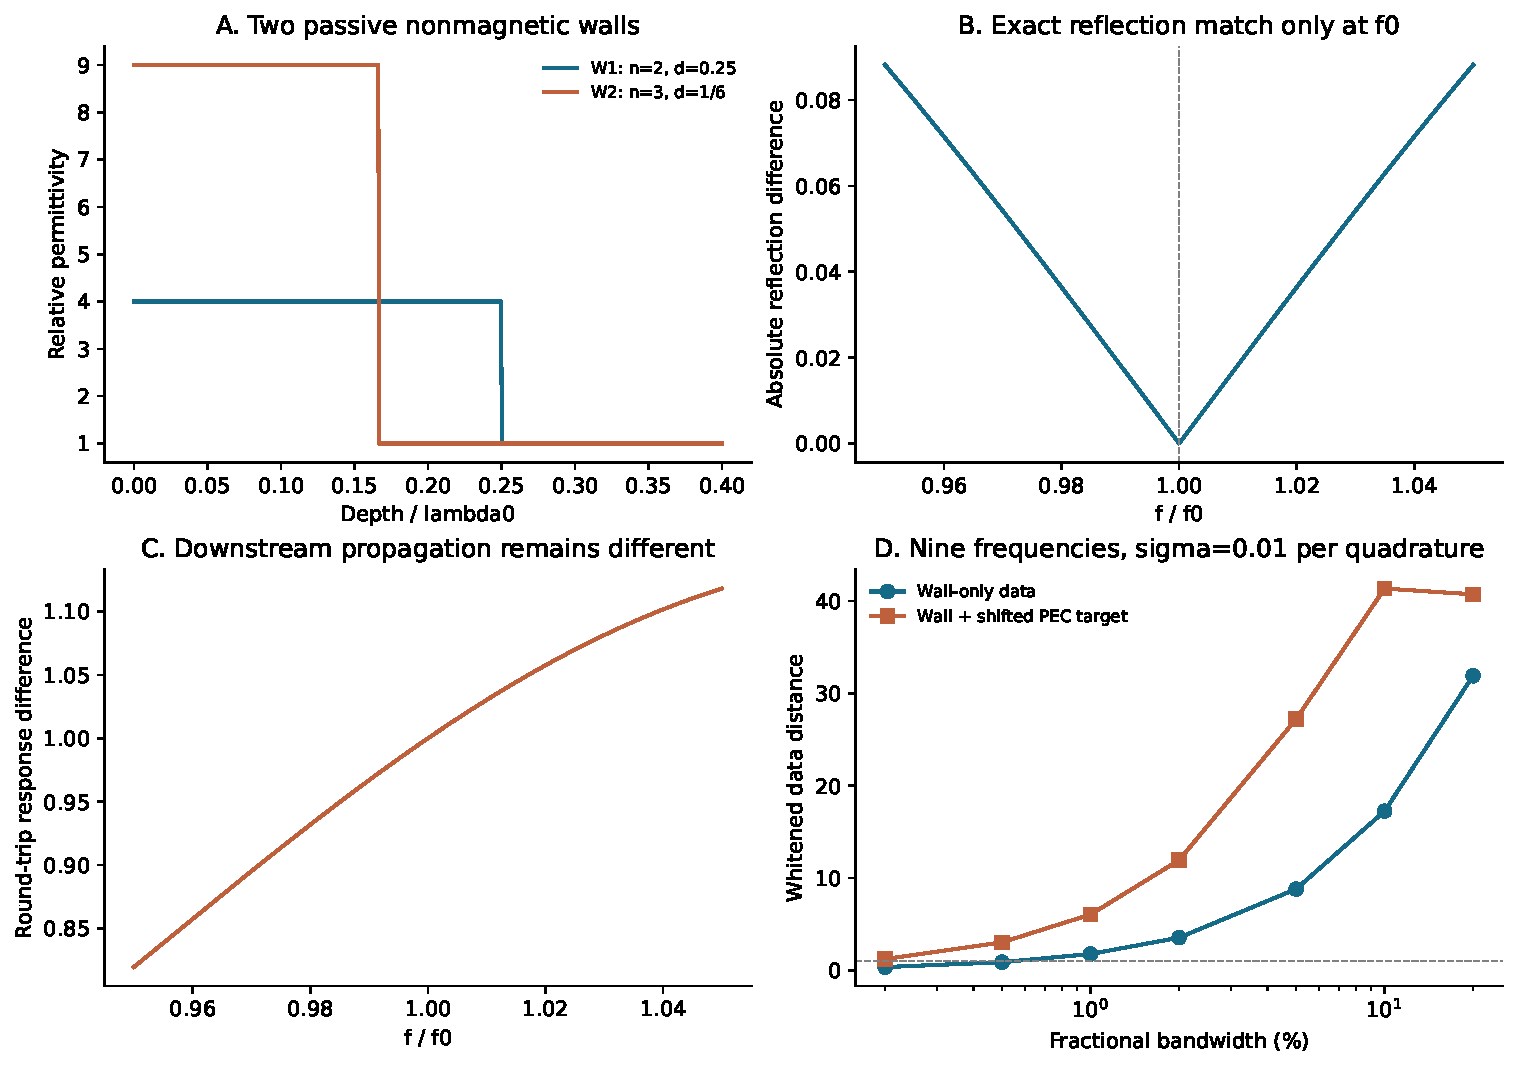
\includegraphics[width=.98\linewidth]{../analytic_results/exact_maxwell_witness.pdf}
\caption{本轮已执行的一维精确 Maxwell 核验。不同厚度的共振板在中心频率反射相同；同参考面双程传播不同。有限带宽破坏该特定联合补偿，不把此图当作二维复杂墙体结果。}
\end{figure}

\subsection{补偿、可辨识充分条件和真正的失败边界}
墙厚与折射率的光程、界面反射幅度、目标位置、复散射强度和仪器相位可相互影响。只有光程近似相同并不足以保证全波数据相同；空腔与等效低介电区也只在特定长波极限近似等效，界面散射、色散与多次反射会打破等效。金属增强结构的路径变化同理，必须计算完整响应。

一种充分条件是总材料 $m$ 在声明数据类中唯一且稳定可恢复，并且 $H(m)$ 在该类上 Lipschitz；则复合映射给任务稳定性。更弱条件只要求任务在纤维上常值。连续边界 Maxwell 数据的部分数据唯一性文献说明，不能笼统说“单侧必然不可辨”；其允许的激励、几何与完整边界响应，远强于有限天线采样。\cite{L_Partial,L_Zhai}

有限孔径在 Born 极限中限制被采样空间频率；全非线性多次散射可能带入附加耦合，也可能恶化 conditioning。因此 Born 缺角结论是机制解释，不能直接充当全非线性严格核空间结论。

另一个独立失败机制是屏蔽：闭合理想 PEC 屏障内的外部不可达目标不能由外部照明恢复；这时相应可测目标响应本身为零。高损耗或高反射层使双程幅度极小，任务 Fisher 信息相应衰减。它与“墙回波相似但透射行为不同”是两种机制，不应混称。

\subsection{错误墙模型如何传递到定位}
在真实世界附近，若强行固定 $\widehat W=W_*+\delta w$，且目标数据映射足够光滑，局部最小二乘给
\[
\delta x\approx J_X^\dagger(n-J_W\delta w).
\]
若相关目标可观测子空间最小奇异值 $s_X>0$，则局部
\[
\|\delta x\|\lesssim
s_X^{-1}\left(\|n\|+\|J_W\delta w\|\right)
+\text{受控二阶项}.
\]
有 nuisance 时须先消去其可补偿分量。带正则时应写 $(J_X^*J_X+\Lambda_X)^{-1}J_X^*$，同时承认 prior 偏差。多个目标模式、目标出现/消失、相位周期歧义或 $s_X\to0$ 时，这个局部界失效。不能只给传播误差一个小数字，就宣称定位误差也小。


\clearpage
\section{传播后验、等价类与概率压缩}
\subsection{强目标所需的传播对象：四块签名}
选择计算任务域注入 $U$，发射 $Q$，物理接收算子 $R$。在固定离散化和参考介质下写
\[
L(W,X)=L_W-U V_XU^*,\qquad G_W=L_W^{-1}.
\]
$V_X$ 是任务域内相对参考材料的对比，包含必要频率因子和质量矩阵；不是任意将物理材料值直接代入。定义
\[
\boxed{\Psi_T(W)=(d_W,A_W,B_W,C_W)}
\]
\[
d_{W,\gamma}=b(\gamma)+R(\gamma)G_WQ(\gamma),\quad A_W=RG_WU,\quad
B_W=U^*G_WQ,\quad C_W=U^*G_WU.
\]
由 resolvent 得精确响应
\[
\boxed{\mathcal F(W,X)=
d_W+A_W V_X(I-C_WV_X)^{-1}B_W.}
\]
后文为简洁将 $d_{W,\gamma}$ 记为 $d_W$；其余各块也隐含相同的 nuisance。不同 $\gamma$ 不能在压缩时被忽略。先用物理复线性算子构造四块，再对最终观测实化白化；一般实协方差的白化未必为复线性。若把白化吸收进 $R$，则全部相关算子须采用一致实化表示。

四块分别描述已有背景响应、任务域到接收、发射到任务域及任务域经环境返回的自反馈。只保留 $RG_WQ$ 或某个单程 Green action，不能控制强目标造成的反复散射；只保留 Born 核 $A_W V B_W$ 则对应弱目标近似。这里的分式响应属于标准 T-matrix/Schur 结构，A17-X 已研究相近端口对象与有限反馈，本报告不作恒等式原创声明。\cite{L_Tmatrix,R_A17X}

\begin{proposition}[强目标传播误差的条件上界]
对两个环境及声明任务类中的每一个 $V$，假定
\[
\|V\|\le v,\quad\|(I-C_iV)^{-1}\|\le\beta^{-1},\quad
\|A_i\|\le a,\quad \|B_i\|\le b,\qquad \beta>0.
\]
记各签名块差异为 $\delta_d,\delta_A,\delta_B,\delta_C$。则
\[
\boxed{\|\mathcal F_1(V)-\mathcal F_2(V)\|
\le \delta_d+\frac{bv}{\beta}\delta_A+
\frac{av}{\beta}\delta_B+
\frac{abv^2}{\beta^2}\delta_C.}
\]
\end{proposition}
\begin{proof}
令 $T_i=V(I-C_iV)^{-1}$。精确恒等式
\[
T_1-T_2=T_1(C_1-C_2)T_2
\]
与分解
\[
A_1T_1B_1-A_2T_2B_2
=(A_1-A_2)T_1B_1+A_2(T_1-T_2)B_1+
A_2T_2(B_1-B_2)
\]
给出结论。
\end{proof}
该上界的物理限制比公式本身更重要：$\beta$ 必须对正在压缩的目标类有效。接近墙--目标耦合共振时，$\beta\to0$，内部块误差可按 $\beta^{-2}$ 放大。小材料距离、接收小残差或一个 well-conditioned reduced core 均不能替代这一条件。本命题处理共同计算域上的有界体对比；PEC、阻抗或实体边界变化需要相应 trace/边界版本，不能直接令 $v=\infty$ 沿用此界。前述 PEC 解析反例有独立的精确级联推导。

若任务输出有物理单位，上界各范数必须使用相容的源/场/材料 metric；白化可吸收进 $R$。多频多源可用加权直和范数。仅保存有限探针的响应时，上述 $\delta$ 只有探针意义，推广到连续任务类另需覆盖或概率嵌入界。

\subsection{材料后验向传播响应的推送}
\[
W\sim\mu_W^y\quad\Longrightarrow\quad
\Psi_T(W)\sim(\Psi_T)_\#\mu_W^y.
\]
这比存储完整稠密 Green 矩阵更符合任务，但必须保留其与 $X,\gamma$ 的联合依赖。$\Psi_T$ 的维数仍可能很大，尤其 $C_W$ 覆盖任务域内部全部场自由度时。

一般有
\[
G_{\E[W]}\ne\E[G_W],\qquad
\E[\mathcal F(W,X)]\ne
\mathcal F(\E[\Psi_T(W)],X).
\]
第一式来自求逆非线性；第二式还含 $V(I-CV)^{-1}$。即使未来观测对 $H$ 线性，平均响应也仅给出均值，遗漏
\[
\operatorname{Cov}(Y\mid y)
=\E[\operatorname{Cov}(Y\mid W,y)\mid y]
+\operatorname{Cov}(\E[Y\mid W,y]\mid y)
\]
中的分支间项。多峰分布不能由均值矩阵完整表示。

平均 Green 不一定对应原材料类中的任何局部本构。它在某些共同边界条件下可能仍有线性、互易等性质，不能笼统宣称平均一定违反物理；真正问题是它一般不能代表原来的非线性混合测度。

\subsection{任务等价与近似聚类}
固定目标类 $\mathcal V$、收发配置和噪声，定义
\[
d_T(W_1,W_2)=\sup_{V\in\mathcal V}
\|\mathcal F(W_1,V)-\mathcal F(W_2,V)\|_{\Sigma^{-1}}.
\]
这是一种伪度量。$d_T=0$ 给出真正等价关系；$d_T\le\varepsilon$ 不具传递性，不能把阈值近邻自动命名为数学商空间。实践中应使用半径或直径受控的覆盖、聚类或量化。

相同四块签名是任务等价的充分条件，未必是必要条件：未被任务激发/观测的端口自由度和内部表示变换可能不影响任何允许响应。以任务响应定义等价可避免把内部 gauge 错当物理区别。

对固定弱目标类，只保留有限 Born response kernel 可能足够；对强目标类则需要内部反馈或直接的全非线性任务响应。因此“材料结构不同、传播等效”依赖任务，不存在对所有目标、频率和极化通用的廉价标签。

\subsection{保持原联合先验的后验压缩界}
令 $v=(X,\gamma)$，允许原先验 $\pi_0(dw,dv)$ 相关。真实及近似后验定义为
\[
d\mu=Z^{-1}e^{-\Phi(w,v)}d\pi_0,\qquad
d\widetilde\mu=\widetilde Z^{-1}e^{-\widetilde\Phi(w,v)}d\pi_0.
\]
例如用代表 $c(w)$ 的传播签名计算 $\widetilde\Phi(w,v)$，但仍保留每个原始 $w$ 的 prior 质量和 $v\mid w$ 条件结构。

\begin{proposition}[联合测度不变时的概率误差]
若 $|\Phi-\widetilde\Phi|\le\varepsilon$ 在原先验几乎处处成立，则
\[
e^{-\varepsilon}\le\frac{\widetilde Z}{Z}\le e^\varepsilon,
\qquad e^{-2\varepsilon}\le\frac{d\mu}{d\widetilde\mu}\le e^{2\varepsilon},
\]
从而有保守界
\[
\boxed{\|\mu-\widetilde\mu\|_{\TV}\le\tanh\varepsilon.}
\]
同一界控制目标边缘分布、任何目标事件的概率，以及使用相同未来预测核的预测分布。
\end{proposition}
证明及尾部处理见附录。该概率扰动原理已有成熟先例；Research W 可争取的贡献在于 Maxwell 任务误差是否能有效、低成本地进入该界。\cite{L_Cotter,L_Lie,L_Zahm}

对于白化 Gaussian likelihood，若
$\|F-\widetilde F\|\le\delta$ 且 $\|y-F\|\le R$，则
\[
|\Phi-\widetilde\Phi|\le R\delta+\tfrac12\delta^2.
\]
结合四块签名界得到一条可证明但条件性的链：
\[
\text{传播块误差与稳定裕度}
\ \Longrightarrow\ \delta_F
\ \Longrightarrow\ \varepsilon_{\log L}
\ \Longrightarrow\ \text{目标后验误差}.
\]
残差 $R$ 在高维白化空间通常与 $\sqrt{\dim y}$ 同阶，因此简单 uniform 界可能非常保守。只有证书在实际噪声和预算下有非平凡宽度，才有算法价值。

若误差界仅在 $C$ 内成立，必须保留
\[
\|\mu-\widetilde\mu\|_{\TV}\le
\mu(C^c)+\widetilde\mu(C^c)+\tanh\varepsilon.
\]
候选库之外的质量不能凭“没有找到”设为零。若不掌握两侧尾质量，就只能报告条件误差证书。

\subsection{联合相关性为何不能被聚类丢掉}
若
\[
\mu(dw,dv)=\mu_W(dw)\mu(dv\mid w),
\]
对墙体分簇 $C_j$，定义
\[
p_j=\mu_W(C_j),\qquad
\mu_j(dv)=p_j^{-1}\!\int_{C_j}\mu(dv\mid w)\mu_W(dw).
\]
则
\[
\mu_v=\sum_jp_j\mu_j
\]
完全精确。用一个代表墙体 $w_j$ 的条件分布替代整个 $\mu_j$，会产生额外误差
\[
\left\|\mu_v-\sum_jp_j\mu(\cdot\mid w_j)\right\|_{\TV}
\le\sum_jp_j\|\mu_j-\mu(\cdot\mid w_j)\|_{\TV}.
\]
相近 Green 签名不自动控制这个项，尤其当 $p(v\mid w)$ 有结构相关性。最稳妥的实现是保留联合粒子 $(W_i,X_i,\gamma_i)$，只共享数值传播表示，随后用一致 likelihood 校正。

另一个常见错误是先用同一 $y$ 得到 $p(W\mid y)$，再计算
\[
p(W\mid y)\,p(y\mid W,X)\,p(X\mid W).
\]
这会比正确 joint posterior 多乘一个 $p(y\mid W)$。正确条件分解包含
\[
p(X\mid W,y)=
\frac{p(y\mid W,X)p(X\mid W)}{p(y\mid W)}.
\]
若初始墙体来自真正独立的校准数据，则可以按条件 Bayes 顺序吸收后续新数据；不能把同一观测换名字后当独立校准。

\subsection{“写入传播模型”的决策应是任务风险}
给定任务签名 $H$ 的平方损失，
\[
R(h\mid y)=\E[\|H(W)-h\|_T^2\mid y].
\]
不要求 $h$ 可由某个材料实现时，最优为 $\bar h=\E[H\mid y]$，且
\[
R(h\mid y)=\operatorname{Var}_T(H\mid y)+\|h-\bar h\|_T^2.
\]
若必须选择合法环境 $\widehat W$，则求到 $\bar h$ 最近的可实现签名，或选择 posterior medoid。它不会消除不可约的传播方差。

“安全固定”应限定为：对声明目标任务，使用 $\widehat W$ 的额外风险不超过预算。若 $R\le\epsilon^2$，仅由 Markov 可得
\[
\Prob(\|H-H(\widehat W)\|_T>t\mid y)\le\epsilon^2/t^2.
\]
它不是无条件频率覆盖保证。低概率而高损失的分支宜用事件损失、尾风险或 CVaR；材料逐像素 $95\%$ 置信不控制此类联合尾事件。

如果一个遗漏传播模式有真实后验质量 $\alpha$，且与固定模型任务距离至少 $b$，则风险至少为 $\alpha b^2$。但从未校准的候选库中无法可靠计算 $\alpha$。这解释了残差很小却过度自信的机制，也解释了为什么事后只重加权不能恢复被置零的模式。

\begin{longtable}{p{28mm}p{120mm}}
\toprule
动作 & 合理触发条件\\
\midrule
Accept & 对当前任务，数值、传播压缩与尾风险均在预定预算内；接受的是受限制的传播近似。\\
Keep branches & 当前数据难分，而下游响应差异超过容差；保留联合分支与条件目标样本。\\
Revisit & 新的全模型核验发现偏差、共振裕度失效、出现新传播模式，或任务区域改变；恢复自由度并重建表示。\\
Acquire & 用户允许新增观测时，期望任务风险下降超过采集和计算成本；新数据不参与当前被动结果的选择。\\
\bottomrule
\end{longtable}

\subsection{概率体积、局部强方向与未知拓扑权重}
优化残差给的是点值。对局部弱坐标 $z$ 和强坐标 $s$，真正的边缘后验为
\[
p(z\mid y)\propto\int
e^{-\Phi(s,z)}p_0(s,z)\,ds.
\]
定义 $\Psi(s,z)=\Phi(s,z)-\log p_0(s,z)$、$s_*(z)=\argmin_s\Psi(s,z)$ 及 $H_{ss}=\partial_s^2\Psi(s_*(z),z)$。若强方向有单个内点极小值、近似 Gaussian 且高阶余项受控，Laplace 近似才给
\[
p(z\mid y)\approx
e^{-\Phi(s_*(z),z)}p_0(s_*(z),z)
(2\pi)^{d_s/2}\det H_{ss}(z)^{-1/2}.
\]
只优化 $s$ 会漏掉条件厚度及 determinant；边界、多极小值或奇异方向下须重新积分，不能自动取“半 Gaussian”。参数变换的体积因子取决于所声明 prior 的基准测度；如果在 latent 中已有正确 prior，不能再凭直觉乘一个 Gram determinant。

固定 continuation 轨迹在高维连续 posterior 中通常是零测度对象。端点残差接近并不赋予相同概率，也不证明连接轨迹有重要质量。F3 已验证自然参数线段可在端点合格时仍离开竞争似然范围；P2 未建立稳定跨拓扑模式，均应作为本研究约束。\cite{R_F3,R_P2}

\subsection{同一份数据可以迭代使用，但不能重复计证据}
合法方法包括以同一 posterior 为不变分布的 block Gibbs/MH、同一目标的坐标优化，以及 tempering SMC：
\[
\pi_\beta(u)\propto\pi_0(u)e^{-\beta\Phi(u)},\qquad
w_i^{\,k+1}\propto w_i^{\,k}
e^{-(\beta_{k+1}-\beta_k)\Phi(u_i)}.
\]
最终 $\beta=1$，各增量和为 1。相反，反复 $\pi_{k+1}\propto\pi_k e^{-\Phi}$ 会得到 $\pi_0e^{-(k+1)\Phi}$，相当于虚构更小噪声。

将数据按频率、时间窗拆块时，只有条件独立或明确使用联合条件密度，才能直接乘 likelihood。由相同原始数据得到的早/晚门控结果往往相关；需要联合协方差。由 $y$ 确定的初步图 $\widehat m(y)$ 不是新的传感器证据。

在精确推断、同一 prior、同一数据和合法计算下，联合反演、Gibbs 交替、分块消元或多假设递进应指向同一个后验。不同效果只能来自近似、求解稳定性、模式混合、算力分配或新增采集。


\clearpage
\section{Green 更新、A17 接口与四类误差}
\subsection{精确背景更新及其真实计算条件}
令 $L'=L+\Delta L$，$G=L^{-1}$。在相关逆存在时，
\[
G'=G-G\Delta L(I+G\Delta L)^{-1}G.
\]
它不需要 Neumann 级数收敛；若使用级数截断才需要相应小量条件。接近极点时，有限逆仍可能存在但条件数很大，截断或低秩近似可能失效。

若 $\Delta L=U K V^*$，则可使用 Woodbury 小核
\[
G'=G-GU(I+K V^*GU)^{-1}K V^*G.
\]
秩为 $r$ 时，需要相应 $r$ 个传播作用及 $r\times r$ 的小系统。若变更涉及 $q$ 个材料体素，标量离散的秩通常至多 $q$，三维矢量场可能约为 $3q$ 或由边/面自由度决定。一个标量同时改变全域介电率可使 $\Delta L=\alpha M$ 满秩；\textbf{材料 latent 的维数不是算子更新秩}。

小支撑、远场端口分离、窄任务类和重复查询可能带来可压缩结构；强共振、金属网络、细皮肤层及频率变化可能破坏它。低秩是否存在需在实际 input/output 与误差范数中测量，不能由“局部更新”直接推出。

通常只需要 $GQ,GU,G^*R^*$ 等 actions，而非完整 $N\times N$ Green 矩阵。尤其四块签名的 $C=U^*GU$ 会成为大成本：若 $U$ 覆盖任意未知目标的整个域，端口数可与场自由度同阶。此时全矩阵缓存并没有降阶。

\subsection{局部墙变化怎样同时改变四种任务传播}
在同一固定 nuisance 下，令 $U_S$ 注入被修改区域，$U_T$ 注入任务域，$\Delta L=U_SKU_S^*$，定义
\[
M_S=K(I+C_{SS}K)^{-1},\qquad C_{SS}=U_S^*GU_S.
\]
再令 $R_S=RGU_S$、$B_S=U_S^*GQ$、$C_{TS}=U_T^*GU_S$、$C_{ST}=U_S^*GU_T$。四块签名的有限更新精确满足
\[
\boxed{
\begin{bmatrix}\Delta d&\Delta A\\\Delta B&\Delta C\end{bmatrix}
=-\begin{bmatrix}R_S\\C_{TS}\end{bmatrix}
M_S\begin{bmatrix}B_S&C_{ST}\end{bmatrix}.}
\]
此式是标准 resolvent 的任务端口限制，也是理解 A17 双侧反馈的自然接口；其代数并非新颖。当前无目标数据只检验 $R_SM_SB_S$，而强目标还需要另外三个乘积。因此 $R_SM_SB_S$ 很小不控制 $C_{TS}M_SC_{ST}$；局部区域可以在当前照明/接收下较暗，却经任务域返回的场参与内部反馈。

若有人在任意矩阵空间中找到 $M_S$ 使第一个乘积为零、其他乘积非零，这仍不是合法墙体反例：$K$ 必须来自允许的局部、共享频率、被动 Maxwell 材料更新，且 $M_S$ 与 $K$ 的非线性关系不能被忽略。完整反例必须同时满足这些约束。若只在一阶取 $M_S\approx K$，结论也只能是一阶的。

对一个固定强目标，可把上述 $G$ 换成含该目标的 $G_X$ 再求墙变化。目标会改变两侧的激发和接收场，所以 wall-only 与 target-present 的可见性不一致；这既可能形成传播风险，也可能让联合观测更容易区分墙体。本轮带宽实验显示了后一种情况。潜在设计原则是同时筛查当前数据项与任务反馈项，不是只寻找辐射弱的材料方向。

\subsection{A17 的可迁移内容及其限度}
在固定材料状态下，令 current basis 为 $V$，
\[
R_V=V(V^*LV)^{-1}V^*,\qquad
\bar C=(I-R_VL)C,\qquad\Gamma_C=C^*L\bar C.
\]
对任意任务输入 $B_T$ 与输出 $O_T$，同一 Galerkin 增广给出
\[
\boxed{
H_{V+C}-H_V=
O_T\bar C\,\Gamma_C^{-1}
C^*(B_T-LR_VB_T).}
\]
这是 A17 的 $Y_C\Gamma_C^{-1}N_C$ 的直接 input/output 泛化。它解释新增电流须同时被任务激发并返回任务输出，才对该任务有效。原始输入、保留空间反馈与输出可见性各自不同。\cite{R_A17,R_A17core}

要区分两种“暗”：
\begin{enumerate}
\item $SC$ 很小而 $S\bar C$ 显著：原 current 直接辐射弱，但经保留反馈可见。这是 A17 的具体机制。
\item 某材料方向 $h$ 满足 $DF(m)h\approx0$，而 $DH_T(m)h$ 显著：这是观测任务与下游任务不一致。必须包括材料注入及传播，不能仅由 current 列 $O_TC$ 推出；它不是同一个定理。
\end{enumerate}

同一个 $[V,C]$ 上，Schur 写法与普通 Galerkin 的解相同；A17-X/P2 已有机器精度核验。\cite{R_A17X,R_P2} 因而不可能普遍证明“A17 的代数写法在同空间上比最优 Galerkin 更准”。潜在贡献只能来自空间选择、数值稳定性、误差估计或计算组织，并与允许相同缓存和输入信息的对照比较。

\subsection{真实墙体更新不能直接套用冻结 paired support}
A17/A12 的 paired material support 对共同 $L,B,r,\Lambda$ 下的指定 current 近似改变成立。墙体材料真正改变时，$L$、总场依赖的材料注入 $B$、残差 $r$ 都改变。

在共同实材料坐标的无约束 GN 二次子问题中，定义
\[
h_i=J_i^*r_i+\ell_i,\qquad
H_i=J_i^*J_i+\Lambda_i,\qquad s_i=-H_i^{-1}h_i.
\]
若 $J_1=J_0+D$、$r_1=r_0+\delta r$，则
\[
\Delta h=D^*r_0+J_0^*\delta r+D^*\delta r+\delta\ell,
\]
\[
\Delta H=J_0^*D+D^*J_0+D^*D+\delta\Lambda,\qquad
s_1-s_0=-H_1^{-1}(\Delta h+\Delta Hs_0).
\]
这些是 GN 二次模型的差分，不是完整非线性目标 Hessian 的公式。即便 $D=Y\Gamma^{-1}N$，还会出现 $J_0^*\delta r$ 等新作用；active set 变化也需重新处理 KKT 条件。原 paired support 描述局部更新差在哪里，不是错误墙体锁定的安全保证。

原 A17-X 已推导有限局部材料提案下的双侧反馈修饰、端口残差和小核扰动界；Research F 已给 primal--dual 与 likelihood 误差接口。\cite{R_A17X,R_F} Research W 再次写出这些代数只能作为复用，不构成新章节的原创核心。

\subsection{数值传播误差：可检验的 primal--dual 界}
求解 $LE=Q$，近似为 $\widetilde E$，令
\[
r_p=Q-L\widetilde E,\qquad
r_d=O^*-L^*\widetilde Z.
\]
则精确恒等式
\[
OE-O\widetilde E=
\widetilde Z^*r_p+r_d^*L^{-1}r_p.
\]
若已验证 $\sigma_{\min}(L)\ge\alpha>0$，经 dual 修正后的误差满足
\[
\|OE-O\widetilde E-\widetilde Z^*r_p\|
\le\frac{\|r_d\|\|r_p\|}{\alpha}.
\]
这是既有 goal-oriented residual 代数。它可用于四块签名的 task-restricted action，不必估计整个 Green 算子。

关键是 $\alpha$ 是否有可靠又便宜的下界。一个可能入口是预条件算子 $M$ 满足经验证的 $\|I-ML\|<1$，从而
\[
\|L^{-1}\|\le \frac{\|M\|}{1-\|I-ML\|}.
\]
只抽查几个向量、观察 reduced core 条件数或用经验 held-out 误差，不能给出这个 uniform 上界。用完整 SVD 获得下界也可能比直接求解更贵。条件失败表示该证书无效，不代表完整 Maxwell 解不存在。

\subsection{四类误差必须分账}
\begin{longtable}{p{27mm}p{54mm}p{67mm}}
\toprule
误差 & 数学对象 & 可用控制与不可替代项\\
\midrule
数值近似 & 同一 $m$ 下的离散、迭代、ROM、截断误差 & 网格收敛、后向残差、dual/inf-sup；不能核验材料是否真实。\\
错误固定模型 & $\mathcal F(m_*)-\mathcal F(\widehat m)$ & 需要真实世界或有覆盖意义的不确定集合；小求解残差不控制。\\
材料后验不确定性 & $\Psi_T{}_\#\mu^y$ 的分散与多模式 & 联合推断、任务 Bayes risk；它不是数值误差。\\
未建模结构 & 偏离所声明材料/天线/色散类的真实差异 & 独立验证、模型扩展、受约束 discrepancy；不能靠更小迭代 tolerance 消除。\\
\bottomrule
\end{longtable}
可对已明确的两种前向近似使用三角不等式组合，但不能把未知真实模型偏差默认计为零。如果数值误差 $\delta_n$ 和分支压缩误差 $\delta_b$ 都有界，likelihood 误差应使用
\[
R(\delta_b+\delta_n)+\tfrac12(\delta_b+\delta_n)^2,
\]
而非漏掉 $\delta_b\delta_n$ 的两个独立半平方。详见附录。

残差模型 $y=F(m,\gamma)+\xi+n$ 可表达 discrepancy，但任意高自由度 $\xi$ 也能吸收目标信号。应有物理支持或独立数据确定其先验；增大噪声直到候选相容不属于科学验证。

\subsection{值得检验的任务导向 current exchange}
定义一组明确任务及其分布 $\nu_T$，如在查询域内放置不同位置、材料强度和极化响应的合法测试目标。可考虑
\[
\mathcal E(V)=
\E_{\mu_W^y,\nu_T}
\|F_W^{\rm full}(X)-F_{W,V}(X)\|_{\Sigma^{-1}}^2.
\]
选择固定实际 current 秩下的替换 $V\to V'$，以单位完整计算成本的风险下降为准：
\[
\frac{\mathcal E(V)-\mathcal E(V')}{C(V\to V')}.
\]
这与改善某一步材料 GN gap 的目标不同，也与材料 MAE 不等价。

但 $\mathcal E$ 需要 full reference 或可靠误差界，不能免费使用 oracle。可从小候选池出发，用近似评分提出 finalist，再以付费任务 actions 和上下界决定接受；无法证实下降时 no-op。对给定有限候选池，若分数区间可靠且旧空间保留，可保证只接受经证实有正收益的动作；它不保证候选池覆盖全局最优，也不保证同成本胜过普通 task-POD/Krylov。

A17 最新效率审计显示原本预想的 $Jd$ 不是全部瓶颈；bank/anchor/workspace 构建和非线性路径也重要。\cite{R_A17eff} 因而这个分支的第一步应测费用，不应先推测将某个公式降秩就能加速。

\subsection{成本模型与强对照}
设场自由度 $N$、频率数 $N_f$、发射数 $N_s$、更新端口数 $r$。以 $C_{\rm fact}(N),C_{\rm rhs}(N)$ 表示实际后端一次分解与单 RHS 代价。
\[
C_{\rm full}\approx
N_f\big[C_{\rm fact}(N)+N_sC_{\rm rhs}(N)\big].
\]
端口更新需支付 $G U$、接收/伴随 actions、$r$ 核构建与 $r^3$ 解；典型 setup 为 $N_frC_{\rm rhs}$，存储可能为 $O(N_frN)$。dense LU、稀疏 FEM 与迭代 FMM 的成本结构不同，不能一律写成 $O(N^3)$。

ROM 还要付离线快照、基生成、正交化、每个材料下 reduced operator 组装、误差检查和 fallback。总账至少包含：
\[
C_{\rm total}=C_{\rm setup}+C_{\rm proposals}+C_{\rm rejected}
+C_{\rm checks}+C_{\rm fallback}+C_{\rm inference}.
\]
对照必须允许 direct solve 复用 LU 和多 RHS，Krylov 使用合理预条件与 warm start，ordinary Galerkin 使用相同空间，T-matrix 使用真实端口。比较同 current rank 有机制意义，但不等于同费用性能。


\clearpage
\section{递进的合理定义：可回退的计算前沿}
\subsection{场消元与材料推断是不同操作}
对一个固定合法材料世界，把场自由度分成被消元集合 $A$ 和保留集合 $B$：
\[
\begin{bmatrix}L_{AA}&L_{AB}\\L_{BA}&L_{BB}\end{bmatrix}
\begin{bmatrix}E_A\\E_B\end{bmatrix}
=\begin{bmatrix}Q_A\\Q_B\end{bmatrix}.
\]
在 $L_{AA}$ 可逆时，
\[
S_B=L_{BB}-L_{BA}L_{AA}^{-1}L_{AB},\qquad
Q_{\rm eff}=Q_B-L_{BA}L_{AA}^{-1}Q_A.
\]
接收也必须同步更新：
\[
R_{\rm eff}=R_B-R_A L_{AA}^{-1}L_{AB},\qquad
d_{\rm eff}=R_A L_{AA}^{-1}Q_A,
\]
所以
\[
y=d_{\rm eff}+R_{\rm eff}S_B^{-1}Q_{\rm eff}.
\]
只更新 Schur 矩阵而忽略有效源和测量偏置会改变物理问题。

精确场消元是代数重排，合法消元顺序不会改变最终响应。未知材料使
$(S_B,Q_{\rm eff},R_{\rm eff},d_{\rm eff})$ 成为相关随机对象。若还要消去未知材料 $m_A$，则须积分
\[
p(y\mid m_B)=\int p(y\mid m_A,m_B)\,\pi_0(dm_A\mid m_B),
\]
而非把 $m_A$ 固定为一次重建。场自由度消元与材料后验边缘化不能混为同一步。

\subsection{与坐标弱相关的可信任务区域}
为每个物理查询区域 $T$ 及其任务类定义传播风险 $R_T$、数值误差 $\epsilon_{n,T}$、压缩误差 $\epsilon_{b,T}$ 和尾质量上界 $\eta_T$。在指定损失与容差下，定义
\[
\mathfrak F(y)=
\{T:\ R_T\le r_T,\ 
\epsilon_{n,T}+\epsilon_{b,T}\le e_T,\ 
\eta_T\le\eta_{\max}\}.
\]
$\mathfrak F$ 是\textbf{可信任务集合}，不是必然存在的光滑曲面。它可以不连通，可以绕过高损耗区域，也可以因新的全模型核验而收缩。使用物理域、坐标变换后的场范数与材料测度，可避免依赖任意像素编号；有限网格实现仍有离散化误差。

这一构造并未证明可以从有限数据计算出所有风险。若 $\mu^y$ 只由短链或候选库近似、尾质量未知，$\mathfrak F$ 必须标为经验可信集。不能把近似推断的低方差误称严格可观测性。

前沿无需满足 $\Omega_1\subseteq\Omega_2\subseteq\cdots$。材料模式分裂、任务改变、共振出现或新增数据揭露旧模型错误，都可能要求回退。即使真实新增观测存在，Bayes 风险也是在对未来观测取期望意义下非增；某个具体观测可使局部 posterior 更分散。

\subsection{按深度推进何时有额外物理意义}
如果介质几何、源/接收边界与到时满足因果分离，初期响应确实只依赖一个可确定的近层区域，那么 layer stripping 可利用这种三角结构。高空间频率边界恢复、严格凸 foliation、已知初始 focusing function 等都是实质假设。\cite{L_Somersalo,L_Zhai,L_Marchenko22}

在未知倾斜空腔、钢筋网络和折角墙中，散射路径的时间顺序一般不同于 Cartesian 深度。一个近层角反射可以比深层直达回波晚；有限带宽窗有旁瓣与泄漏；墙--目标反复交互使所谓“近层数据”仍包含深层材料。因此本报告不建议预设固定层数和单向锁定。

如果保持全部材料自由度，仅逐步改变分辨率、频率权重或块更新次序，这通常是 FWI 的优化策略。若同时保留后验分支、控制传播压缩和允许回退，则可能有独立计算价值，但必须与直接 joint inference 做消融，而非把所有收益归为“递进”。

\section{推荐算法：联合概率目标不变的传播分支推断}
\subsection{完整目标和两种运行模式}
推荐的算法先以完整总材料 posterior 为目标，再将传播表示作为可替换的数值缓存。它有两种明确输出身份：
\begin{enumerate}
\item \textbf{发现模式：} 有界 multistart、成核和受保护 corrector，输出 full-validated weighted hypotheses 或 candidate ensemble；不提供未经建立的 posterior 概率。
\item \textbf{概率模式：} 在一个可被独立参考检验的先验上运行 SMC/MH，保持正确权重和 nuisance 相关性；有限粒子仍需混合、模式覆盖与校准检查。
\end{enumerate}
首轮 P0 采用第一种，P1 的小维概率基准采用第二种。复杂拓扑全网格 posterior 不是第一轮必须解决的目标。

\subsection{初始化与不固定拓扑的材料表达}
在包含所有可能材料的有限域内使用连续被动场或随机 level-set prior。设候选任务域 $T_j$，不把它们称为已知墙后 mask。未知边界和空气可出现于整个域中；发射接收附近的已知空气区域属于设备几何先验，应单独披露。

确定性初值可采用 free-space/BP、低频正则 joint FWI 或 N3 的合法投影。N3 只在其训练支持和物理接口一致时作为 proposal；原模型针对已知背景，不能直接当未知墙先验 sampler。\cite{R_A26}

概率模式最稳妥的是从原 prior 抽样。如果使用由数据拟合的初始分布 $q_0(u\mid y)$，必须能计算密度、满足 $\pi_0\ll q_0$，并用 $\pi_0/q_0$ 初始化权重，或从明确的 posterior 桥开始。可加入已知正权重的 prior 混合分量保护支持。漏掉 prior 支持的 $q_0$ 不能靠后续 importance correction 自动修复。把数据生成的候选端点等权当 prior 粒子会改变目标。

\subsection{提案：局部、全局与拓扑事件各自承担作用}
在 Gaussian latent 中可用 pCN 保持参考 prior，再由正确 likelihood 接受；对物性/校准参数使用声明坐标中的 MH。局部 GN 或弱方向只用于提高 proposal 的方向性，不宣称正维 exact fiber。

全局提案可使用独立 prior、coarse multiscale block move、随机占据场更新或有显式密度的 birth/death。空腔生成不需预定义 cavity count；连续潜在场穿越临界零水平可改变拓扑，RJMCMC 只是可变维几何表示的一种选择。

物理 corrector 可解
\[
\min_u\ \Phi(u)+\lambda\mathcal R(u)
\quad\text{s.t.}\quad
d_T(\Psi_T(u),\Psi_T(u_{\rm old}))\ge s_T,
\]
并保持一个事先选定的成核核心、材料合法性和进度，防止所有提案被拉回旧点。它适合候选发现；任意多对一投影后的端点不是正确 MH proposal，除非计算其密度、Jacobian 或设计扩展状态可逆核。

\subsection{传播风险驱动搜索}
对已有库 $\mathcal A_K$，一个发现目标可定义为
\[
\max_{u\in\Theta_{\rm admissible}}
\min_{a\in\mathcal A_K}d_T(\Psi_T(u),\Psi_T(a))
\]
并约束完整数据竞争度、prior 合法性及物理尺度。它鼓励发现新传播行为而非仅新外观。不能只最大化几何距离或像素差异。

这个目标搜索的可能是低概率极端世界。若要声称发现“重要模式”，还需邻域质量积分或独立 posterior 样本，而不是只看点 prior 密度或 $\Delta\Phi$。QD/RL 分数可影响提案与预算，不能替换 Bayes 权重。\cite{R_G,R_F3,R_P2}

为防止指标过拟合，应有与构建库不同的任务 probes 做核验；若这些 probe 依赖未来真实观测，则只能作为后续采集评估，不能进入当前被动在线选择。对模拟 probe 可预测但无观测，这属于计算任务定义，不是新增信息。

\subsection{完整伪代码}
\begin{quote}
\textbf{输入：} 原始多静态观测 $y$、联合噪声 $\Sigma$、总材料与 nuisance prior $\pi_0$、任务类 $\mathcal T$、完整求解器及固定费用上限 $B$。\\
\textbf{输出：} 当前目标推断、传播代表、原联合样本/候选身份、误差与未覆盖质量状态。

\begin{enumerate}
\item 固定所有物理约定、任务损失、prior、频率和审计协议；保存同一 observation identity。
\item 获取廉价确定性 anchor 供提案使用。概率模式另从 $\pi_0$ 抽样，或正确加权已知 $q_0$；记录所有初始化费用。
\item 建立 $\pi_{\beta_k}\propto\pi_0e^{-\beta_k\Phi}$ 的温度序列，$0=\beta_0<\cdots<\beta_K=1$。用增量 $\Delta\beta$ 更新权重；条件 ESS 仅决定数值调度，不当模式覆盖证明。
\item 对每个联合粒子/候选求完整共享材料 Maxwell 状态，或使用有界数值替代；对所有源、频率、极化使用同一材料世界。
\item 计算 task-restricted $\Psi_T$ actions 及稳定裕度。选择少量物理代表，使估计的加权传播误差最小；保留原联合粒子与簇内条件分布。
\item 运行局部 pCN/MH、全局提案与可选拓扑事件。candidate corrector 的结果单独入发现库；未经密度修正，不直接并入 posterior 粒子权重。
\item 用传播近似加速 likelihood 计算；若证书不能决定接受/拒绝则付费 full solve。无严格证书时使用合法 delayed acceptance 或完整 likelihood，保留近似误差记录。
\item 以任务风险执行 Accept / Keep branches / Revisit。Accept 只共享当前任务的数值传播表示，不删除原 prior 支持；Revisit 恢复被缓存的完整状态或产生全局提案。
\item 每次材料、任务域或稳定裕度显著变化后重建传播表示；以相同原始数据进行联合全 Maxwell 校正。若有新增观测，另按联合条件 likelihood 更新。
\item 达到 $\beta=1$ 后检查目标统计量的链间一致性、重要模式与参考误差、独立预测及完整费用。预算到达仍未收敛则输出候选/近似状态及未解决项。
\end{enumerate}
\end{quote}

\subsection{数值近似怎样不破坏概率目标}
若每个状态的 $\Phi$ 有可验证区间，可用同一个随机阈值 $\log U$ 与包含 prior 和 proposal 项的\emph{对数 MH 比}上下界比较：下界足以接受或上界足以拒绝时结束，否则提高求解精度。对固定离散目标，这种 lazy evaluation 不改变接受决策；连续 PDE 与离散化误差仍须另审。

没有严格误差界时，固定 surrogate 的 delayed acceptance 也可保持完整离散 posterior，要求 $\widetilde\pi$ 在 $\pi$ 支持上为正。两阶段比率分别为
\[
r_1=\frac{\widetilde\pi(u')q(u\mid u')}
{\widetilde\pi(u)q(u'\mid u)},\qquad
r_2=\frac{\pi(u')\widetilde\pi(u)}
{\pi(u)\widetilde\pi(u')},
\]
总接受概率为 $\min(1,r_1)\min(1,r_2)$；proposal 只在第一阶段计入一次。每次通过第二阶段仍需 full likelihood；不能声称无代价。若 surrogate 随链状态自适应，必须满足相应自适应 MCMC 条件或分阶段冻结，不得随意忽略适应性。

SMC 使用 surrogate 权重时必须明确每阶段 target。若
\[
\widetilde\pi_k\propto\pi_0e^{-\beta_k\widetilde\Phi_k},
\]
则阶段权重应乘
\[
\exp[-\beta_{k+1}\widetilde\Phi_{k+1}
+\beta_k\widetilde\Phi_k],
\]
而非在 surrogate 改变后仍只乘 $\exp[-\Delta\beta\,\widetilde\Phi_{k+1}]$。最终转到完整 target 再乘
$\exp[-\Phi+\beta_K\widetilde\Phi_K]$。只有中间粒子确实正确加权到声明 target 时，这一校正才成立；不能靠最后一次 full likelihood 补救任意历史权重错误。高 ESS 不证明先前遗漏模式已恢复。最初 hard discard 的模式如果 proposal 无正支持，最后校正无法找回。

\subsection{停止条件与开销控制}
固定数据下，停止不是“已经看到所有深度”。合理停止条件是：任务 posterior/候选覆盖在预算内不再有经核验改进；压缩风险低于任务容差；或者现有数据已给出无法降低的任务歧义见证。

每个阶段都可触发 NO-GO：full solver 已比 ROM 更便宜；任务稳定裕度过小导致证书无用；posterior 模式质量无法参考验证；发现的传播差异对实际目标损失无影响。遇到这些结果应收紧研究问题或结束分支，不能自动扩大 rank、网络、带宽或 prior 来制造成功。

在有限 $K_p$ 粒子、$K_g$ 传播代表、$N_f$ 频率、$M_T$ task probe 下，昂贵项约为
\[
K_pN_f\left(C_{\rm fact}+N_sC_{\rm rhs}\right)
+K_gN_f C_{\rm port}(M_T)
+C_{\rm proposals}+C_{\rm verification}.
\]
压缩只有在 $K_g\ll K_p$ 且传播差异允许共享、setup 可摊销时才可能节约。这个条件本身就是需要测量的假设。

\subsection{主动测量作为独立扩展}
真正新增采集设计 $a$ 可用期望任务 Bayes risk 减少量
\[
U(a)=R^*(y)-\E_{y_a\mid y,a}R^*(y,y_a)-C_{\rm acquisition}(a).
\]
它针对目标损失，而非单纯墙像素 entropy。跨频 gain、位置和材料色散应共享 nuisance；不能为每个候选未来频率选择不同物理世界来伪造不可区分性。

主动策略必须与固定较高频、固定极化/位置以及简单等预算扫描比较。Research B 已显示复杂选测未稳定超过强固定频率对照。\cite{R_B} 因此它是可选后续，不应拿新增观测收益替被动递进算法背书。


\clearpage
\section{既有研究证据、可复用接口与不可跨越的边界}
\label{sec:prior-evidence}

\subsection{证据版本与本轮实际读取范围}

本轮以五个用户仓库的原始文档为证据，读取日为2026年10月22日。读取源为GitHub文件接口；没有重新运行这些历史物理实验，也没有将仓库发布、软件检查或代数回放等同于独立Maxwell验证。下表固定本轮引用版本；正文的数值结论是对原始记录的核验与归纳。\cite{R_A17,R_A26,R_A30,R_B1,R_C1}

\begin{longtable}{p{1.2cm}p{5.3cm}p{6.85cm}}
\hline
简称 & 仓库 & 固定commit\\
\hline
\endfirsthead
\hline 简称 & 仓库 & 固定commit\\\hline
\endhead
A17 & a17-maxwell-certified-exchange & {\scriptsize\texttt{df61a1b533682a883cdaf65259b4528c354bd832}}\\
A26 & a26-om-feedback-prior-completion & {\scriptsize\texttt{2603f3bd16c48e48587fedc4363975779def17f5}}\\
A30 & a30-maxwell-observable-material-manifold & {\scriptsize\texttt{717d3d26a290248bd2b9aeb55f3d03694b407b84}}\\
B1 & b1-probabilistic-maxwell-imaging & {\scriptsize\texttt{064d0aaed9772cadd573866eec84f159895b317b}}\\
C1 & c1-physics-state-generative-imaging & {\scriptsize\texttt{83056881e89329212b16f5be47a4d0dbc4465943}}\\
\hline
\end{longtable}

\textbf{完整审读的核心记录。}
A17的旧决策、closure入口、最终中文closure报告、论文主文件、CORE\_THEORY和CONDITIONAL\_EXCHANGE\_THEORY，以及最新效率报告；A26的README和最终决策；A30的E0/E1决策；B1总入口、Joint P2决策、最新P2材料fiber报告与理论修订、F与F3实施报告、Research A/B/T/G实施报告、LXZ实施报告、A17-X/F3竞争审计；C1入口与P2决策均已全文审读。长文件首次输出有截断时，补读相关原文后才采用结论。

\textbf{取得全文但只审读重点章节。}
A17技术补充主文件未展开审读全部输入子文件。Joint P2完整报告的物理目标、补偿、概率参考、C1和下游交接主体已读，核心数值再用完整决策交叉核对。A17-X原Pro报告已取得，重点复核第4--5节有限端口与双重反馈、第7节多源材料可实现性、第9节动态误差；Research F原Pro报告重点复核第6--7节材料几何与有限延拓、第9节目标残差、第11节概率测度。这些重点阅读不写成整份原报告逐段独立验证。\cite{R_A17X,R_F}

\textbf{未取得独立原文的部分。}
本轮未直接取得Research L/Z/X各自完整ZIP及P3-L完整报告；B1中以P3-L和strong-direction搜索未找到相应原稿。LXZ实施报告已经直接读到，其上游阅读记录不能代替本轮读取。A12、A24--A25、A27--A29、A31的独立全稿也未逐一取得；A12的paired结论可由A17正式理论与历史对照核验，其余只按用户任务书及已读实施报告的历史引用使用。P3-L仅作为用户指定的理论方向，不能补造其证明或实验数字。

\subsection{必须更新的A17判断：有限重建正例已经出现，但仍未建立加速}

根目录旧A17\_DECISION把非线性重建列为NOT\_RUN；这不能再概括后来的closure。最终closure在十个完整额外对象上报告：对象汇总的完整GN二次gap中位比为0.492818，即下降约50.7\%。99个计划单元中96个有审计结果，95改善、1相同；1个失败和2个未运行保留在计划分母中。额外对象有历史研究暴露，准确描述是规则锁定后的额外对象验证，不能写成完全新盲测。\cite{R_A17}

三组完整受约束反演中，receiver与exchange采用相同初始化、材料表示、先验、LM调度、可行域和完整非线性Armijo检验；测得结果如下。它们提供有限重建后果，不能从局部gap自动推出。\cite{R_A17}

\begin{longtable}{p{3.1cm}p{3.9cm}p{2.5cm}p{3.1cm}}
\hline
对象／表示 & 复材料相对误差 & 相对下降 & 完整耗时比\\
\hline
\endfirsthead
\hline 对象／表示 & 复材料相对误差 & 相对下降 & 完整耗时比\\\hline
\endhead
平滑／voxel & \(0.3027\to0.2699\) & \(10.84\%\) & \(2.68\)\\
近接触／Gaussian & \(0.6722\to0.6707\) & \(0.22\%\) & \(1.74\)\\
壳体／Gaussian & \(0.6096\to0.5660\) & \(7.16\%\) & \(1.46\)\\
\hline
\end{longtable}

近接触的实部稍差；第四对象没有完成成对基线，不能把失败前缀当作完整比较。有限噪声检查72个单元中71改善、1不动，仍只支持指定对象、状态与噪声范围。严格输出误差半径尚不存在，原论文已经将实现定位为verified conditional exchange，而非确定性认证。

最新效率后续采用每轮只检查第一名、最多三次接受和精确geometry-only缓存，在两个规定对象上相对原exchange减少26.89\%和9.64\%耗时；相对receiver-only仍为1.958和1.318倍，结论保持CONDITIONAL。更值得Research W吸取的是成本归因：完整\(Jd\)只占原exchange净增量的1.19\%和3.82\%，反复构建bank、anchor及工作空间才是主要费用之一。因而再造一个verification ROM不一定击中瓶颈。\cite{R_A17eff}

历史负结果没有被覆盖：paired材料修复胜过指定direct current enlargement，但同实秩材料Krylov更强；paid paired耗时约为匹配PCG的1.416倍，记录的RHS从66增至342；宽域从零选择材料相关电流也没有普遍超过receiver起点。Research W可以借用条件设计思想，必须重新证明其对传播任务的效用与完整费用。\cite{R_A17}

\subsection{A26、A30与最新P2：容量、可行性、选择与速度必须分开}

\textbf{A26的负结果是网络增量负结果。}
三个CNN相对各自物理初值，在复杂三家族上有约23--24\%材料改善；匹配31,810参数和2,000次更新时，显式feedback模型N2相对N1、N3的改善分别约为\(-0.225\%\)、\(-0.273\%\)，区间跨零。完整warm推理为较快对照的3.274倍。这个事实不能抹去A17后来的有限重建正例，两者检验的机制不同；也不能将N3视为后验采样器、原材料先验内合法anchor或未知墙体的已验证重建器。\cite{R_A26}

\textbf{A30严格区分表示容量与在线选择。}
Sparse-64的35.69\%、PCA-64的21.91\%是读取truth进行参数拟合的离线容量；完整candidate convex hull有13.12\%改善，但同bank的实际L-weighted mean恶化3.32\%。29个合法补偿对的最小完整白化距离为8.84，复杂条件最小9.18，未达到原协议的清晰到模糊转变；uniform误差证书也未通过。这些是已实现搜索与参数化的负结果，不是全局补偿不存在的证明。\cite{R_A30}

\textbf{最新P2支持有限噪声替代，不支持新拓扑生成优势。}
24个新对象只有15个得到相容physics-only anchor，held-out为4/8。69个替代解释是跨24份观测的archive计数；held-out只有1个达到原结构尺度的替代，稳定拓扑事件改变为0。全部8个held-out的基础MAE为0.06513030，联合archive的Best-of-4为0.06424926，约1.35\%只是oracle诊断，在线默认Selected仍是基础图。更强的sphere-only Full-J及hard-prior对照也能找到替代材料，削弱了软谱机制的独特性；小Gaussian/Flow没有独立收益。\cite{R_P2}

P2还直接检验了A17-X求值。相同空间的Schur和直接Galerkin差约\(1.91\times10^{-15}\)；A17的setup摊销耗时59.490ms，optimized full为5.346ms，约11.1倍。A17的fallback为17/48，goal-ROM为4/48；该fallback使用已保存full prediction检查误差，是离线oracle辅助审计，不能描述为可部署的在线误差控制。exact T使用真实256-cell ROI，66维latent不被当成66个物理端口。\cite{R_P2}

\subsection{从A12到P3-L的用途映射}

\begin{longtable}{p{1.7cm}p{5.7cm}p{5.7cm}}
\hline
方向 & 已核实结果／可复用内容 & Research W的限制\\
\hline
\endfirsthead
\hline 方向 & 已核实结果／可复用内容 & Research W的限制\\\hline
\endhead
A12/A17 & 指定current改变的双侧材料步差；受条件核验的同秩设计。 & 固定quadratic包含关系不保证truth风险、posterior质量或等成本优势。\\
A24--A29/N3 & A26直接支持廉价先验网络作为强对照；历史反馈增量失败保留。 & 未直接重读全部各代原稿；known-background二维结果不直接覆盖未知墙。\\
A30 & 35.69\%离线容量与在线选择失败并存。 & 不得truth-selected candidate、oracle weights或未来观测泄漏。\\
A31 & 用户指定的被动性、能量、互易性与材料风险区分。 & 本轮未直接核验A31全文；物理约束不等于结构唯一性。\\
B1/Joint P2 & 同一连续先验中的事件积分、共享gain与条件样本交接；径向补偿见证。 & 四维同心支持不是任意未知拓扑；多个事件不一定是分离modes。\\
C1 & 小型蒸馏MDN事件MAE约0.0132，条件CDF误差约0.142--0.162。 & 完整连续后验目标未达；state/memory无稳定增量，先不扩训练。\\
Research A & 每观测3--10个径向候选；静态结构分层有离线Best4收益。 & 在线最小residual不改善；正例主要来自结构分层，非A17归因。\\
Research B & 正确joint-history、跨频共享nuisance与候选缺漏stress。 & 复杂选测未稳定胜过固定3.2；漏中心孔family后29/30未报警。\\
Research T & 不预设总孔数的局部空气成核可被full-grid补偿为相容端点。 & 32相容端点记录不等于32独立模式；候选材料MAE约0.49--0.51，成像未改善。\\
Research G & post-corrector novelty、archive与失败记录可复用。 & 仅一个近阈值支撑扩张，非新洞；Best4未改善，不支持现在训练RL。\\
Research F/F3 & 正确商先验、材料几何、有限反馈、非零进度corrector。 & 三个weak端点彼此很近；九个插值中点均超竞争阈值；高阶方法无同成本增量。\\
Research L/Z/X & LXZ实施区分局部与全局核，C1提案经正确MH可用。 & 新显著结构为0；hybrid不优于简单global；独立原ZIP未在本轮取得。\\
A17-X & 有限端口、双重反馈、source-shared材料可实现性及tail界。 & 七维latent可产生575秩更新；同空间不能优于ordinary Galerkin精度。\\
P3-L & 局部弱几何与strong-direction概率厚度是用户指定后续问题。 & 未找到原报告，不能补造已证明定理或已执行实验。\\
\hline
\end{longtable}

上述映射分别依托A17/A26/A30、Joint P2/C1、A/B/T/G、F/F3、LXZ和最新P2原文。\cite{R_A17,R_A26,R_A30,R_B1,R_C1,R_A,R_B,R_T,R_G,R_F,R_F3,R_LXZ,R_A17X,R_P2}

其中有两条对Research W特别重要的教训。第一，T的不同候选都进入同一95\%噪声球，但与base之间仍相差约6.24--14.27个白化单位；数据相容不等于两世界统计不可区分。第二，F3的合法端点不能保证连接路径相容，局部弱方向也不能自动跨拓扑。传播分支探索必须重新验证有限完整响应，不能由Jacobian核或漂亮材料图推断成功。\cite{R_T,R_F3}

T的记录跨轮相关，而且使用更宽的full-grid复材料box。LXZ实施报告明确指出，相应补偿破坏了旧P0的固定phase约束；所以不能把这些端点当成原固定相位prior内已发现的重要后验模式。允许拓扑变化、满足宽材料box、保持同一个概率prior，是三项不同要求。\cite{R_T,R_LXZ}

\subsection{A17可迁移的精确内容，以及Research W新增的误差项}

在固定材料、总场注入、残差与先验下，A17定义
\[
R_V=V(V^*LV)^{-1}V^*,\qquad
\bar C=(I-R_VL)C,
\]
\[
Y_C=S\bar C,\quad
N_C=C^*(B-LR_VB),\quad
\Gamma_C=C^*L\bar C.
\]
当core与Schur可逆、使用严格Galerkin及一致实化时，
\[
J_C-J_0=Y_C\Gamma_C^{-1}N_C,\qquad
s_C-s_0\in H_0^{-1}\operatorname{Range}[J_0^*Y_C,N_C^*].
\]
这里\(B\)包含真实材料本构导数与当前total field；所有照明共享实材料变量。该结果适用于同一个固定、无约束材料quadratic，不能无说明地推广到active constraints改变。\cite{R_A17core}

任意任务输入\(B_{\mathcal T}\)和输出\(O_{\mathcal T}\)可替代原注入与receiver：
\[
H_{\mathcal T,V+C}-H_{\mathcal T,V}
=
O_{\mathcal T}\bar C\,\Gamma_C^{-1}
C^*(B_{\mathcal T}-LR_VB_{\mathcal T}).
\]
这是标准Schur推论。它提供一个清楚接口：以目标区域、未来探测源及目标风险选择current空间；单凭换成任务输出，不构成独立新定理，也不比同空间ordinary Galerkin更准。

\textbf{墙体材料更新还改变残差与注入。}
若真实背景改变导致\(J_1=J_0+D\)、\(r_1=r_0+\delta r\)，则
\[
\Delta h
=D^*r_0+J_0^*\delta r+D^*\delta r+\delta\ell,
\]
\[
\Delta H=J_0^*D+D^*J_0+D^*D+\delta\Lambda,\qquad
s_1-s_0=-H_1^{-1}(\Delta h+\Delta Hs_0).
\]
因此即使\(D\)具有A17的低秩因子形式，旧paired支撑还一般需要加入\(H_0^{-1}J_0^*\delta r\)；先验变化再产生额外方向。固定current表示的改善，不能替代错误墙假设、传播后验分歧或模型外误差的控制。

\subsection{避免与自己已有A17-X/F报告重复}

A17-X原Pro已把局部材料端口写成
\[
P=R_0U,\quad H=U^*GP,\quad O=SP,\quad B=U^*E_0,\qquad
\Delta F=O(I-DH)^{-1}DB.
\]
本段\(R_0=L_0^{-1}\)是完整anchor逆，\(G\)是内部背景Green，不能与上一节Galerkin算子混同。这里四个端口对象和局部T-matrix已经存在；一维latent也可能使材料算子变化满秩。它还已给出双重反馈修饰的有限exchange：
\[
\Delta F_{V+C}(D)-\Delta F_V(D)
=[S+O_VQ_VU^*G]\bar C\Gamma_C^{-1}N_UQ_nB,
\]
其中\(Q_V=(I-DH_V)^{-1}D\)，\(N_U=C^*(U-L_0R_VU)\)，\(R_U=U-L_0R_VU\)，新空间的相应有限反馈记为\(Q_n\)。其端口残差
\[
\rho_D=R_UQ_VB,\qquad
\Delta F_F-\Delta F_V=SL_1^{-1}\rho_D
\]
及在\(\|Q_V\|\epsilon_H<1\)下的有限误差上界，也已在旧报告第5节提出。W可以将这些对象用于wall--target接口，但不能重新命名为首次发现。\cite{R_A17X}

Research F原报告第9节同样已有primal/dual恒等式。若近似状态\(Z\)的残差为\(R=B-LZ\)，近似dual为\(\widetilde\Psi\)，
\[
R_d=O^*-L^*\widetilde\Psi,\qquad
OL^{-1}B-OZ
=\widetilde\Psi^*R+R_d^*L^{-1}R.
\]
若已验证完整算子的稳定性下界\(\beta\leq1/\|L^{-1}\|\)，余项不超过
\[
\|R_d\|\,\|R\|/\beta.
\]
这只控制数值近似误差。Reduced core条件数、浮点backward residual、经验留出误差不能代替完整Maxwell稳定性界，也不能控制漏掉的墙体后验模式。\cite{R_F}

因此Research W真正可能独立的问题是：\textbf{当前有限观测所保留的材料等价类，是否决定完整目标相互作用所需的传播对象；若不决定，如何量化不能消除的任务风险，并压缩其联合后验。} 同一套resolvent代数可作工具，新的科学结论必须来自可辨识性、概率压缩或同完整费用的任务效用。

\subsection{对下一轮实验的直接约束}

最小实验应先用固定材料支持、频率、孔径、噪声和nuisance构造两世界，检验当前数据近等价是否伴随\emph{完整墙加同一目标}响应差异。单程Green差别可能在往返中抵消；仅画单程差不能证明墙后成像风险。多解marginalization与递进调度必须分开消融。所有方法允许相同factorization、多RHS、Schur复用及合理Krylov策略；计入basis准备、拒绝、dual、fallback与端到端费用。

如果只能形成candidate archive，则报告candidate-only；只有明确目标测度、权重、校准与覆盖诊断之后才报告后验近似。正确MH形式不意味着短链已经混合。Joint \(p(W,X,\gamma\mid y)\)压缩时必须保留传播变量与\(X,\gamma\)的相关性；不能先以同一\(y\)生成\(p(W\mid y)\)，又将同一likelihood不经条件分解地乘一次。这些要求直接来自既有B1/F3/P2失败，已经足以排除“先扩大网络、再期待自动出现多解与加速”的实施顺序。\cite{R_B1,R_F3,R_P2}


\clearpage
\section{文献与原创性审计：Research W 的可成立边界}

本节核验截止于 2026 年 10 月 22 日。定向检索尚未核实一篇同时完成“未知复杂墙体拓扑、完整 Maxwell 墙--目标多次散射、联合多模态后验、概率传播更新、任务风险控制推进”的论文；这不是穷尽检索或不存在证明。模块组合本身也不足以支撑强原创。最接近本课题的已有工作分别集中在 corrected Green 穿墙反演、Marchenko 单侧重定基面、反射--透射歧义以及目标导向 Bayesian 降维。

\subsection{用户指定十项文献：核验内容与读取范围}

下表明确区分全文核查与摘要核查。关于未取得全文的论文，本报告不据题名外推其定理范围；完整题名、作者和可核验入口列于参考文献。

\begingroup
\small
\setlength{\tabcolsep}{4pt}
\begin{longtable}{p{2.45cm}p{6.05cm}p{5.5cm}}
\hline
文献与读取范围 & 已核实内容 & 对 Research W 的直接限制 \\
\hline
\endfirsthead
\hline
文献与读取范围 & 已核实内容 & 对 Research W 的直接限制 \\
\hline
\endhead
Somersalo 1994\cite{L_Somersalo}；出版社摘要 & 高频时谐 Maxwell；以高空间振荡的边界激励确定表层电磁参数，利用 invariant embedding 向内传递边界数据。摘要指出耗散使方法适于近边界区域。 & 连续边界算子与特殊激励不等于有限单侧天线数据。更新传播边界后继续成像已有明确先例。 \\
\hline
Hesford--Chew 2010\cite{L_DBIM}；作者机构详细摘要 & DBIM 以更新的不均匀背景连续线性化，MLFMA 加速反复正演。指定 PMC 入口受访问限制。 & “反演材料、更新背景、再次反演”属于既有 DBIM/FWI 思想；必须另证任务风险或计算收益。 \\
\hline
Marks 等 2017\cite{L_Marks}；全文 & sparse blind deconvolution 同时恢复目标与圆对称 Green，不必预知平面层厚度及材料；包含 K-band 建材实验。 & 利用层状介质横向对称和目标稀疏性。既非任意墙体拓扑，也非完整非线性联合后验。 \\
\hline
Jakobsen--Tveit 2018\cite{L_Tmatrix}；出版社正文检索 & 频域各向异性导电介质的 DBI T-matrix，体积分方程与背景更新。直接页面访问间歇失败，正文由出版检索入口取得。 & resolvent、动态 Green 和局部 T-matrix 更新不构成新恒等式。2015 年相关工作已比较固定及动态背景\cite{L_Tmatrix15}。 \\
\hline
Watson 等 2024\cite{L_Watson}；全文，重点第 3--7 节 & BEM corrected Green、ROM 与 variable projection；处理 corner-wall 传播及墙介电率 nuisance，保留墙体多次散射。 & 墙形近似已知、标量模型、目标采用 Born 近似；未包含目标间反复散射。是最接近的应用 baseline，不能忽略。 \\
\hline
Zeng 等 2025\cite{L_Lidar}；IEEE 摘要/引言及 BIT 记录 & LiDAR、SLAM、轮廓拟合补偿门窗、柱和凸出结构导致的不规则墙传播；实验改善建筑布局恢复。 & 使用外部精确几何信息，适合作为额外信息对照，不符合本课题无外部墙几何的输入条件。 \\
\hline
Yang 等 2025\cite{L_Building}；IEEE 摘要及作者记录 & 以墙和墙角等结构的连续性建立 Bayesian 建筑内部感知；采用结构变分推断。 & 未核全文；目前核实的规范散射单元模型不足以支持“任意拓扑完整 Maxwell posterior”解读。 \\
\hline
Abugattas 等 2025\cite{L_LayerUQ}；全文重点第 1、2、4、5 节 & 已知层背景的纵波散射，低维参数夹杂，MCMC 展示单频多模态；增加频率可减少部分次模式。 & 是纵波模型，非全矢量 Maxwell；层背景已知。大量正演采样的成本不能直接外推为全网格复杂墙后验可行。 \\
\hline
Minsley 2011\cite{L_Minsley}；USGS 详细摘要 & FDEM 地球物理跨维 MCMC，层数未知，考虑先验及仪器高度不确定性。 & 未知层数已有 Bayesian 解法，但不等价于任意三维孔洞及连通结构；低频导电勘探与 GHz 穿墙条件不同。 \\
\hline
Le Louër--Rapún 2017\cite{L_Topology}；出版社摘要/补充说明 & 三维 Maxwell 拓扑敏感性，分别处理 PEC、腔、阻抗及介质传输问题；检测不预知的个数、位置和形状。 & 拓扑成核已存在；拓扑导数既不是 posterior 权重，也不保证探索重要的全局拓扑模式。本轮未逐页阅读全文。 \\
\hline
\end{longtable}
\endgroup

\subsection{最重要的遗漏先例：Marchenko、前向散射与电磁重定基面}

Marchenko 的目的之一正是从地表反射构造内部虚拟源/接收点及 Green 响应，而无需先精确恢复全部内部材料。Wapenaar--Slob 的多分量单侧表示包含电磁与弹性波框架\cite{L_Marchenko14}。其反射响应是一个具有空间、时间及分量完备要求的算子；初始聚焦场与截断介质的逆透射有关。不能将这个条件替换为“有限单侧数据完全决定内部传播”。原文对因果分离的详细分析与示例主要在一维弹性情形，三维、复杂界面及大偏移下需要额外判断。Diekmann--Vasconcelos 的全波表示进一步处理早期上下行分解的限制；实际求解仍需要初至波估计\cite{L_Marchenko21}。

\textbf{前向散射是 Research W 最相关的缺失信息之一。}van der Neut 等指出，平滑模型直达波代替初始聚焦场会丢失某些前向散射及关联多次反射，并以额外透射数据补回\cite{L_Marchenko22}。其论证与数值例子属于特定声学场景，不能直接升级为普适 Maxwell 非唯一性定理。但它表明“可拟合反射”与“具备正确的下游聚焦场”之间的落差已被明确研究；Research W 必须给出更具体的材料类、有限观测及风险结果。

已有电磁版本也必须纳入审计。Slob--Wapenaar 2017 给出无损三维介质中由单侧地表 GPR 反射构造两个内部点间 Green 的表示，数值例子为一维\cite{L_EM2017}。Slob--Zhang 2016 的有耗三维推导需要两个平行面上的反射与透射，以构造负耗散辅助响应，亦以一维示例验证\cite{L_EM2016}。Yang--Slob 2021 的一维有耗 GPR 反演使用双侧数据，并对反射中的弱耗散作假设\cite{L_EM2021}。有耗声学实验版本同样使用双侧访问\cite{L_Dissipative18}。本轮对这四项核实了作者机构或期刊摘要，不把三维表示存在等同为三维复杂墙实验成功。

因此应将本课题定位为：\emph{当完整反射响应、初始聚焦场、无损性或双侧透射条件不可满足时，识别有限单侧数据仍能确定的下游传播量，并保留无法排除的传播分支。}有限带宽、有限孔径以及未知天线响应不仅是数值截断，也改变可辨识性问题。不能用理想 Marchenko 恒等式替代这些条件下的稳定性证明；也不能将已有单侧 Green 学习重新命名为原创哲学。

\subsection{反射相同而传输不同：已有结论及可争取的新结果}

Waagaard--Skaar 2007 的多模逆散射直接讨论这种歧义\cite{L_Waagaard}。全文第 2 节把一般无损互易单元分解为反射元件与两侧同向模态耦合；若允许反射元件远侧的附加耦合，反射不能唯一确定传输。作者为了实施逆算法，排除该自由度。第 3 节讨论相位及 Takagi 分解歧义；多维类比还带有窄带、耦合结构等限制。它没有解决本课题的一般有限支撑复杂墙问题，但已经覆盖“相同反射不必相同传输”的广泛定性主张。

更早的 Golden 等电磁海冰研究，在一维非磁有耗标量化模型下讨论折射率 $n(x)$ 与电导率 $\sigma(x)$ 联合未知：单个平面波的回波一般不足，底部跳变可提供类似透射的信息\cite{L_Golden}。这里本轮核查的是论文第 II 节及其引用关系，未重新证明所引旧定理。尤其不能照抄其书目误差：Chaderjian 的相应论文实际发表于 1994 年；出版社摘要的唯一性假设是固定波速及点源响应，使用两个平面波分量\cite{L_Chaderjian}。不同激励集、已知参数及界面假设改变结论。

据此，以下内容只能列为数学工具或明确假设下的推论：数据纤维上任务量恒定的因子化判据；局部条件 $\ker DF\subseteq\ker DH$；线性分式的墙--目标反馈表示；一般两点统计下界。它们不能仅因套用于 Green 就宣称为新的 Maxwell 定理。较强贡献需要在\textbf{普通非磁、被动、有界、有限支撑材料类}中完成以下至少一项：有限非线性且物理可实现的近数据等价构造；对带宽、孔径、噪声和 nuisance 显式敏感的任务传播模数；或在实际采集设计下可检验的充分条件。任务应覆盖目标的完整反馈响应，而不只比较一次源到目标传播。

\subsection{目标导向概率、降维与自适应前沿的已有基础}

Lieberman--Willcox 2014 已直接针对预测量而非完整参数场进行非线性 Bayesian inference\cite{L_NonlinearGoal}；Spantini 等 2017 在线性高斯问题中给出目标后验均值、协方差及风险意义下的最优低秩近似\cite{L_Goal}。因此“材料不同但任务等价”和“只保存任务重要方向”不是新理念。Cui--Marzouk--Willcox 的 likelihood-informed parameter and state reduction 同时压缩参数与 PDE 状态\cite{L_Cui}；A17 的 paired material/current space 不能以“双空间”本身作为独立性依据。

Zahm 等以 log-likelihood 梯度统计及适当测度不等式认证非线性后验降维误差\cite{L_Zahm}。Cotter--Dashti--Stuart 以及 Lie--Sullivan--Teckentrup 已建立确定性或随机前向误差到后验误差的理论\cite{L_Cotter,L_Lie}。Research W 可贡献的是可计算、目标相关的 Maxwell 误差证书及其应用条件，而不是重新发现通用 Bayesian 稳定性。数值误差证书也不能认证未被采样到的真实墙体模式。

Calvetti--Nakkireddy--Somersalo 2020 的题目即为 Bayesian filtering layer stripping\cite{L_BayesStrip}。本轮核实其出版记录，未取得全文，因而仅据此否定“概率化剥层从未出现”这一宽泛说法。未知 Green 的跨维 Bayesian 估计也已用于地震多通道反卷积\cite{L_GreenBayes}；不应声称 Green posterior 本身首次出现。

几何推进同样有边界控制与凸叶状分解先例。Zhai 2026 的 dynamical Maxwell 局部唯一性使用严格凸波速 foliation\cite{L_Zhai}；Brown--Marletta--Reyes 的部分边界唯一性对系数边界邻域等条件有明确要求\cite{L_Partial}。本轮核查了相应摘要，不能将连续局部边界 Cauchy 数据与有限天线阵列混同。若本课题的“可信前沿”允许分裂、回退，它更适合作为全局后验的计算预算分配规则；除非另有新数据，不能声称推进创造了信息。SOM 本身也早有二维层状穿墙应用\cite{L_SOM}。

\subsection{四条论文路线：独立性、成本与停止门槛}

\begingroup
\small
\setlength{\tabcolsep}{4pt}
\begin{longtable}{p{2.0cm}p{4.25cm}p{4.05cm}p{3.7cm}}
\hline
路线 & 值得争取的主贡献 & 已被覆盖的弱版本 & 实验门槛与主要风险 \\
\hline
\endfirsthead
\hline
路线 & 值得争取的主贡献 & 已被覆盖的弱版本 & 实验门槛与主要风险 \\
\hline
\endhead
I：传播可辨识性与不可能性 & 合法复杂墙类的有限非线性反例、任务传播模数及 nuisance 补偿后的定位风险界；给出何时任务可辨的条件。 & 两端口相位歧义、一般纤维/kernel 判据、通用 Le Cam 及理想匹配磁性平板。 & 优先 P0。必须用普通材料且经独立全波核验；只有单频教具反例不足。理论独立性最好，TAP 价值取决于 EM 具体结果。 \\
\hline
II：概率 Green 与递进推断 & 受预算约束的分支保留、压缩和回退，改善目标风险/覆盖率，并分离多解与推进的增量。 & DBIM 加 ensemble、SMC 换名；多次使用同一 likelihood；像素置信度硬固定。 & 待 I 支持。须同数据、先验和正演成本比较直接联合推断；模式覆盖与校准最难。大网络不是第一步。 \\
\hline
III：A17 任务反馈计算电磁 & 目标激励、观测及内部反馈共同决定 current enrichment；以传播误差证书和同成本 Pareto 为依据。 & Schur/Woodbury 改名；把 full-GN 指标换名为任务；低维 latent 被误当低秩更新。 & 与现有 A17 最连续，但独立性风险高。须胜 Krylov、标准 goal-ROM、T-matrix；共振/非正规性可能消除低秩收益。 \\
\hline
IV：概率 redatuming & 对无法从单侧数据固定的 direct/forward focusing field 保留物理分支，只输出可辨的内部任务响应。 & 对已有 Marchenko 输出简单蒙特卡洛，未处理聚焦场缺失信息。 & 可作 I 的应用路线；必须显式处理有限孔径、损耗及未知目标，不引入不可获得的双侧数据。 \\
\hline
\end{longtable}
\endgroup

\textbf{推荐顺序。}先检验路线 I 的物理命题，再决定是否值得发展路线 II 或 III。路线 I 的可发表主张应写成“指定材料类和实际有限测量设计下，给出目标传输函数的不可辨识构造或可计算稳定性边界”，而非“首次发现反射不能决定传播”。若现实先验与完整联合数据使所有高概率墙体解释在目标任务上几乎等价，则多墙传播学习不再是主要瓶颈，适宜停止扩大算法规模；若差异确实存在但在线搜索无法覆盖，应先报告可辨识性或搜索负结果，不能以 oracle candidate/weight 替代成像性能。

\clearpage
\section{决定性实验：先找可证伪见证，再比较算法}
\subsection{本轮已执行与尚未执行}
已执行的是第 3 节的一维非磁共振板精确核验、完整 PEC 目标级联以及有限带宽扫描。代码使用 NumPy/解析传输矩阵，没有训练、没有昂贵 Maxwell campaign，也没有运行新的二维或三维反演。

以下 P0/P1 是\textbf{预先定义的下一轮协议建议}，不是实验结果。其阈值是立项门槛，必须在新数据与随机种子生成前冻结；失败后不能移动阈值或增大噪声来救故事。

\subsection{六类场景如何服务不同命题}
\begin{longtable}{p{12mm}p{41mm}p{58mm}p{31mm}}
\toprule
场景 & 内容 & 主要判别机制 & 优先级\\
\midrule
A & 均匀介质墙 & 参考面、相位、背景模型与全波一致性 & 已有一维核验；二维回归\\
B & 未知数量/形状空腔 & 空气成核、局部补偿与 prior 支持 & P0 主场景的一部分\\
C & 倾斜/曲面/厚度变化 & 几何--定位补偿与固定深度失效 & P0 主场景\\
D & 未知层数与材料混合 & 表示能力与数据选择的分离 & P1 后验证\\
E & 导电夹杂/钢筋 & 屏蔽、共振、秩增长及网格误差 & 后置压力测试\\
F & 数据近等价而传播不同 & Candidate I 的有限非线性下界 & 第一优先\\
\bottomrule
\end{longtable}
不必先完成六类漂亮图片。P0 用一个 B+C 混合背景寻找 F 类见证，足以决定是否投入概率算法。E 需可靠金属模型和网格，不应成为首轮预算吞噬点。

\subsection{P0-A：解析回归，已经完成}
使用本研究包的 \texttt{analytic\_witness.py}。必须保留同参考平面、双程响应和 target-present 联合验证。通过条件包括：反射零点、目标响应相位差、联合目标位移补偿、lossless unitarity、频带扩展后的距离变化。独立 Fresnel 公式交叉核验与传输矩阵一致到约 $10^{-16}$。

\textbf{该门槛只保证实验定义没有初等错误。} 不把 P0-A PASS 直接当成未知复杂墙体研究 GO。

\subsection{P0-B：最小二维 TM 全波传播歧义见证}
\paragraph{固定物理。}
取 $z$ 不变的 $E_z$ 极化、$\mu=\mu_0$，求解
\[
(\nabla_{xy}^2+k_0^2\epsilon_r(x,y,\omega))E_z
=-i\omega\mu_0J_z.
\]
它是该对称条件下的 Maxwell 标量子问题，保留全部二维多次散射；并非三维矢量结果。

以 $\lambda_0$ 为单位，可取总未知域
$[-2,2]\times[0,3]$，天线位于前侧 $y=-0.3$、横向孔径 $3\lambda_0$。固定 4 个发射位置与 12 个接收位置，全都位于同一侧。先用 5 个频率 $f/f_0\in\{0.8,0.9,1,1.1,1.2\}$；另有事先冻结的窄带配置用于解释带宽作用，不能看到失败后才改采集。

材料先验覆盖全未知域，不给墙 mask；首轮限制 $1\le\Re\epsilon_r\le9$ 与明确的小损耗范围。逆表示可用 $32\times48$ 全材料/level-set 网格，相关长度、最小可表达特征和边界 prior 全部公开。truth 是一个倾斜且厚度变化的介质体加不规则空气区；这只是固定测试实例，算法不读取其生成类别或孔数。

前向网格须满足预先定义的物理精度，而非只报网格尺寸：至少做一次独立细化和 PML 扩展，要求校准数据误差的白化范数 $\le0.1$，任务响应误差 $\le0.1$；不满足则当前见证不合格。有限几何、频率和损耗要与微分算子及介质界面离散一致，避免 inverse crime。

\paragraph{两种观测合同。}
本实验沿用总场的计算分块：$W=m|_{D\setminus T}$、$X=m|_T$，其中 $T$ 是预先声明的查询域，不是已知墙体边界。在 joint 推断中，$T$ 内允许完整材料，不假设只有一种稀疏目标；传播计算中的背景才将 $T$ 换为参考材料。下述 calibration fixture 额外把 $T$ 实际设为参考材料，供隔离机制使用，这项额外信息不转移到原 joint 任务。
\begin{enumerate}
\item \textbf{Calibration 合同：} 测量时 $T$ 内实际为声明参考介质，比较 $F_{\rm cal}(W_1)$ 与 $F_{\rm cal}(W_2)$。这个合同用于隔离墙传播机制，不宣称现实任务可直接获得。
\item \textbf{Joint 合同：} 使用实际 $F(W,X,\gamma)$，两端允许目标和 nuisance 在相同 prior 内补偿。禁止从数据中减去真实墙或真实目标。它才决定原始 Research W 的适用性。
\end{enumerate}
每份合同必须有独立的 observation identity。源幅和噪声尺度由事先的校准规则固定，对所有被比较方法相同。

\paragraph{任务类和目标函数。}
任务域是前述计算查询域，不假设实际 joint 世界中不存在墙。作为固定的数值任务类，预先给定 12 个空间位置与有限组合法介质材料 $V_X$（例如参考介质内固定尺度圆盘的两种介电对比），并固定对比幅度。评价完整同任务材料全波响应，不能用任意放大 probe 获得巨大 $d_T$。此时 $X$ 是 $T$ 内全部材料，而非与 $W$ 任意相加的语义标签。

可使用局部危险方向提出初猜，再做有限非线性优化：
\[
\max_{W_2\in\Theta_W}
d_T(W_1,W_2)
\quad\text{s.t.}\quad
\|F_{\rm cal}(W_2)-F_{\rm cal}(W_1)\|_{\Sigma^{-1}}\le1,
\]
并限制物理材料范围、弱结构 prior 和最小/最大修改尺度。Joint 合同则直接优化
\[
\min_{X_2,\gamma_2}
\|F(W_2,X_2,\gamma_2)-F(W_1,X_1,\gamma_1)\|_{\Sigma^{-1}},
\]
同时保留真实任务差异（位置、占据事件或强目标传播）。位置/占据必须预先定义为总材料泛函 $q_T(m)$，例如给定对比阈值的占据事件或区域内对比质心；若采用命名物体位置，则需另声明对象生成先验。两个总材料世界必须确实不同，不能仅靠 $\chi_W+h,\chi_X-h$ 的标签重分配达标。$W_1,X_1$ 是声明的参考世界；该构造是可辨识性 adversarial test，不是在线重建性能。

对照为相同预算的普通 Full-J/adjoint、材料匹配随机方向加共同 corrector、multi-start joint FWI。不得把人为阻止普通方法进展的角度约束放入对照。各方法可使用相同 factorization 与 warm-start 权利。

\paragraph{预算与先后顺序。}
首轮只做两个固定背景种子和两种冻结采集配置，先 calibration，再对通过的见证检验 joint。建议整个 P0-B 硬上限为 8,000 complex RHS、2,000 个材料--频率分解和 2 CPU 小时，任一先到即止；40\% 用搜索，30\% 用完整端点/任务验证，20\% 用独立网格，10\% 留失败/重查。具体后端若无法在此预算内完成，缩减场景数量而非把失败费用排除。

这些数值是起始预算，不是理论复杂度保证。只在执行前根据一次公开的 solver benchmark 调整；不能在看到科学结果后重新制定上限。

\paragraph{GO / NO-GO。}
\begin{longtable}{p{24mm}p{124mm}}
\toprule
门槛 & 判定\\
\midrule
机制 GO & 至少一个有限尺寸、非磁、被动、不规则二维 pair：数据均值距离 $d\le1$，事先声明目标类的完整响应有 $d_T\ge3$，并通过独立细化与 nuisance 合法性；报告其是否仅 calibration 成立。\\
原问题 GO & 在 target-present joint 合同下仍有 $d\le1$，且目标任务差异达到事先物理尺度，例如位置差 $\ge0.1\lambda_0$ 或声明占据事件改变；不能用纯墙距离替代。\\
稳健性检查 & 在预定的微小材料/位置扰动下继续检查距离，披露有效范围。孤立精细调谐反例可支持存在性，不能自动支持常见场景算法价值。\\
机制 NO-GO & 所有有限非线性正确器都消去传播差异，或只有错误边界/粗网格/不合法 gain 才满足；停止算法立项。\\
范围 REDIRECT & 仅单频或极窄带成立，实际冻结宽带 joint 配置均不成立：缩为测量充分性/反例边界论文，不继续“通用复杂墙递进”叙事。\\
搜索不确定 & 固定预算没找到：报告 best-found 和失败状态，不能证明全局不存在；但可以据资源决策停止该算法分支。\\
\bottomrule
\end{longtable}

$d\le1$ 对等 prior 固定 Gaussian 两世界意味着最优检验错误率至少 $\Phi_{\rm N}(-1/2)\approx0.309$。这是人为选择的强歧义门槛，不是“95\% noise ball”。$\|y-F\|$ 接近 $\sqrt{\dim y}$ 的两个拟合可有很大相互距离，Research T 的历史结果已说明必须分开。\cite{R_T}

数值容差必须进入门槛。若各端有严格的响应误差上界，应要求
\[
d_{\rm num}+\epsilon_{F_1}+\epsilon_{F_2}\le1,\qquad
d_{T,\rm num}-\epsilon_{H_1}-\epsilon_{H_2}\ge3.
\]
仅观察网格差 $\le0.1$ 不能保护恰好卡在阈值上的见证，也不是连续 PDE 误差的严格上界。若没有可靠误差证书，结论须限定为最细声明的离散 Maxwell 模型，并把网格/PML 检查列为数值一致性证据。

\subsection{P1：区分多解收益与推进收益}
只有 P0-B 支持实际 joint 歧义，才进入 P1。首先用两至数个固定墙分支加少量连续目标/校准参数建立可独立积分的 reference。它检验概率逻辑和压缩界，不声称任意未知拓扑 posterior。原 prior 的分支权重必须明确，后验权重通过 evidence 积分得到，不能用最小残差替代。

\begin{center}
\begin{tabular}{p{29mm}p{55mm}p{62mm}}
\toprule
 & 同时联合计算 & 自适应分块/递进计算\\
\midrule
单点近似 & 正则 joint FWI/MAP & 单点交替更新传播与材料，允许回访\\
多假设 & 直接 joint SMC/MH/参考积分 & 同一 posterior 上的任务风险传播缓存和调度\\
\bottomrule
\end{tabular}
\end{center}
这四格将多假设因素与推进因素分开。Oracle 真墙 Green、错误均匀背景和 free-space 成像另外列为诊断上下参照；它们没有相同可用信息，不能与主方法算“公平胜出”。

主多假设对照使用同一 prior、同一完整 likelihood、相同任务和 proposal 库；优化/提案顺序可以不同，但总费用相同。若多假设已经改善，而递进调度没有进一步改善，应只保留多解传播贡献。

\paragraph{低成本 pilot。}
先 4 个开发背景定参数，再冻结 8 个背景，每背景两份噪声；所有指标以背景为聚合单位。每个方法先锁定相同 full-evaluation-equivalent 上限（建议 256 个多频多源完整前向等价，且同时限实际 wall time），参考积分的费用单列但不免费消失。若短链无法达到参考误差门槛，P1 应判未解决，不用粒子 ESS 冒称校准。

在低维 reference 上，核心 GO 是：重要事件质量及目标 CDF 在固定检查点误差 $\le0.02$；传播压缩保持同一误差目标且实际费用比直接 full 多假设低至少 20\%，或在同费用下显著降低声明任务损失。阈值须在执行前冻结。8 个背景的 coverage 仅作 pilot 描述，不能据少量命中给现实覆盖保证。

\paragraph{必须报告的指标。}
\begin{itemize}
\item 在线决策的目标位置/形状/材料误差；决策为 posterior mean、medoid 或明确 Bayes action，不用 truth-selected Best-of-K。
\item 目标事件概率误差、proper score、校准曲线、可信区间 coverage 及宽度；有独立 reference 才谈概率准确度。
\item 完整目标传播预测误差、四块签名误差与共振裕度；数值误差和环境不确定性分列。
\item 重要模式发现和遗漏、错误固定率、回退次数；无法估计未覆盖质量时填 unknown。
\item 原始全 Maxwell 数据一致性、留出测量误差、所有失败状态。
\item 总时间、峰值内存、分解/RHS、basis/setup、全部拒绝与 fallback；同 rank 不替代同费用。
\end{itemize}
Best-of-K 可以作为明确离线容量诊断，但不能成为在线性能主指标。A30、Research A 与 P2 已表明这个区别足以改变科研结论。\cite{R_A30,R_A,R_P2}

\subsection{独立检验压缩证书与 A17 价值}
为四块签名构造若干受控误差，分别比较仅透射、Born 核、完整四块、普通 goal-ROM 与 A17 条件 enrichment。包含远离共振和接近共振两类；必须允许证书在后者失效。

用实际 full target response 验证上界是否保守、是否错误声称安全，以及界的求值是否比 direct solve 更贵。若只有完整 reference 已知时才能决定 fallback，称为 offline audit；不得把它包装为在线控制。P2 已有这一失败先例。\cite{R_P2}

A17 分支只有在完整总费用对强 direct/Krylov/goal-ROM 存在任务误差--成本 Pareto 改善时继续。若相同空间数值相同、额外选空间却更贵，即停止其优势主张；这不推翻 A17 的冻结机制结果。

\section{现实测量的最低条件与三维推广}
\subsection{不存在脱离任务的统一最低频段}
需要的带宽、孔径和 SNR 应由目标任务距离、材料损耗和 nuisance 共同确定。均匀已知介质中的近似距离分辨率
\[
\Delta z\approx\frac{c}{2B\sqrt{\epsilon_r}}
\]
只能作为量级参考；未知弯曲路径、色散、多次散射和介电误差会改变定位。横向分辨率也依赖角覆盖与距离，不能从中心波长给出普遍数值。

实际最低合同应包括：稳定且可建模的发射谱；复相位可追踪的多静态数据；噪声/相关性估计；阵列位置与时间零点的不确定范围；至少能使已知环境下的目标任务可测的 SNR。若连 Oracle 真墙条件下都无法区分目标任务，研究环境学习没有可挽回的观测信息。

墙内衰减可用路径积分作局部解释：单程幅度约 $e^{-\int\alpha ds}$，往返目标响应约 $e^{-2\int\alpha ds}$；相应均值导数平方的信息量可按 $e^{-4\int\alpha ds}$ 衰减。这是传播路径近似，复杂共振或旁路需 full Maxwell。更高频率可能增加分辨率，也增加衰减与模型敏感性，不能预设总是更好。

\subsection{单侧、多静态、极化与门控}
主验证保持所有天线在同侧。多静态与多极化可改变可达/可观测子空间，但若硬件相位或极化通道缺校准，也增加 nuisance。比较须保留真实通道协方差和重复采集的总能量/时间预算。

早时门控只有在目标最早响应确实晚于保留窗口、且有限带宽泄漏有界时，才可近似得到墙主导数据。未知外表面、侧向绕射、薄层共振和墙--目标耦合会破坏分离。门控丢弃数据通常不会增加信息；它可以改善数值动态范围，但要在 likelihood 中计入剩余模型误差和噪声相关性。

不存在准确 CAD/LiDAR 时，传感器位置本身仍需相对坐标参考。可以把配准误差作为 nuisance；不能既不测量又假定完全准确。额外 LiDAR、背面接收或已知反射体只能作为明确新增信息实验，不能偷偷成为原问题前提。\cite{L_Lidar}

\subsection{从二维 TM 到三维全矢量}
四块签名、Schur/resolvent、推送后验和统计下界可在相应 Hilbert 空间/离散向量系统中保持形式。三维需要重新解决：
\begin{enumerate}
\item $H(\mathrm{curl})$ 相容离散、散度约束、矢量 Green 自项及边界条件；不能逐像素独立标量拟合后称矢量一致。
\item 多源多极化共用同一张量/标量材料场与色散模型；current proposal 必须共同可实现。
\item 对金属的皮肤深度、表面电流与连通网络；高导电极限不能直接沿用粗二维参数。
\item 更大的端口秩、factorization 与预条件成本，非正规/共振对误差估计的影响。
\item 开放有限孔径的三维边缘绕射和出平面泄漏，它们可能消除二维歧义，也可能创造新歧义。
\end{enumerate}
因此二维 PASS 只支持机制继续验证。最终 TAP 若主张一般建筑穿墙，应至少有一组有限三维矢量、同侧采集的物理验证；没有则题名和结论应限定二维。


\clearpage
\section{最终科研判断与可发表贡献的选择}
\subsection{是否值得成为独立 IEEE TAP 主线}
\textbf{有条件值得，但当前应立项为范围受限的理论与机制研究。} 未知环境给目标推断带来的传播歧义，是独立于材料 MAE、局部 current 近似和单点重建的科学对象。这个对象与天线采集、全波多次散射、有限孔径和实际穿透损耗直接相关，具备 TAP 的物理基础。但“通用未知墙体自主递进成像框架”目前缺少三个必要证据：有限尺寸复杂墙中的重要传播歧义、可实际覆盖这些解释的推断方法、以及同费用目标风险改善。

因此本报告建议先给路线 I 一个有硬上限的 P0，而不是直接给整套算法一个长期项目。若 P0 成功，再把一个最有用的风险界与最小概率实验合成论文；若只有理想单频板的歧义，应发表或记录有限结论，而不是用复杂系统包装它。

\subsection{六个候选命题的独立性排序}
\begin{longtable}{p{23mm}p{64mm}p{61mm}}
\toprule
候选 & 本轮能够建立的内容 & 仍决定原创性与价值的缺口\\
\midrule
I：下游可辨识性 & 纤维判据、局部必要/条件充分性、非线性歧义模数、严格一维见证及二点风险下界。 & 在普通有限支撑复杂墙、有限单侧宽带和 nuisance 下给非平凡构造或上界。最高优先。\\
II：传播等价类 & 任务伪度量、四块签名、联合 prior 不变时的 likelihood--posterior 压缩界。 & 找到明显少于材料模式数的传播代表，同时保留目标条件依赖；证书必须实际可计算。\\
III：安全更新 & 任务 Bayes risk、尾质量与错误固定机制；明确确定性模型不能逼近连续材料全后验。 & 非保守的在线证书和模式覆盖。未覆盖质量未知时，不能称绝对安全。\\
IV：A17 任务反馈 & 可复用双侧增广公式、paired support、局部更新四块端口分解。 & 胜过普通 goal-ROM、同空间 Galerkin、优化 direct/Krylov 的实际选空间价值；已有 A17-X/F 覆盖大量代数。\\
V：自适应前沿 & 随机 Schur 四元组、可回退可信任务集合；不依赖预设平面层。 & 计算定义不自动形成新物理定理；需证预算调度对同一 posterior 有独立增量。\\
VI：传播驱动搜索 & 用任务响应新颖度代替像素新颖度，约束完整数据和合法 prior。 & 极端可行点不等于重要概率模式；全局拓扑发现与质量估计仍未解决。\\
\bottomrule
\end{longtable}

最有希望的组合是 \textbf{I 为核心，II 为建设性结论}：先刻画观测不能消除哪些传播差异，再证明哪些差异允许被压缩。III 是其决策解释，VI 是寻找反例和模式的实验工具。IV、V 不必进入首篇论文标题。

\subsection{三条主路线的投入与收益判断}
\paragraph{路线 I：可辨识性与不可能性论文。}
理论对象清楚，能以少量严格见证和数学界检验，而不依赖大规模 posterior sampler。最好的结果不是再给一个反射/透射不同的例子，而是证明一个随频率、孔径、噪声和 nuisance 变化的任务稳定性边界，且构造满足普通材料和全波约束的有限扰动。数值门槛最低，原创潜力最高；失败风险是物理先验和完整联合数据消除所有实用尺度歧义，或所得现象完全落在已有多模逆散射/Marchenko 条件讨论之内。此时仍可得到采集充分性结论，但须改变主张。

\paragraph{路线 II：概率 Green 更新与递进算法论文。}
最终可能最接近用户希望的成像系统，但它需要可靠模式质量、目标条件分布和复杂拓扑支持。其最强卖点应是相同观测与费用下目标风险或概率准确度改善；仅有更多候选、更小数据残差或更漂亮图像不足。当前 P2/F3 证据说明全局搜索与在线选择是瓶颈，直接上 Flow/Diffusion 不能解决这个逻辑缺口。先在可独立积分的低维分支基准上验证概率压缩，再扩展全材料场，是更可信的门槛。若多假设有效而推进无效，应把论文改为不确定环境的 joint inference，不保留无收益模块。

\paragraph{路线 III：A17 任务导向计算电磁论文。}
可直接复用最多现有代码与理论，但独立性审计最严格：A17-X 已有有限反馈端口形式，Research F 已有对偶误差接口，标准 goal-ROM 已优化输出而非全场。新的价值必须在具体选空间原则、可计算误差证书、或经总费用验证的 Pareto 优势。可先用一个目标域、几个合法传播分支和固定 rank 做微基准。若普通 Galerkin 同空间完全一致，而 A17 选空间更贵，必须停止“反馈代数自身更高效”的叙事。小核很精确也不能证明墙体正确。

\paragraph{可选路线 IV：概率 redatuming。}
将无法由有限单侧数据确定的初始聚焦/前向传播作为随机物理状态，研究内部 Green 响应的可辨部分，可能连接到成熟 Marchenko 文献。其优势是问题与波动物理贴近；风险是如果最终仍需不可获得的透射或已知 direct field，就离开原问题。建议作为路线 I 的文献和应用分支，不在当前并行启动第二套大算法。

以上新颖性和 TAP 适配性是本轮判断，不是期刊接受保证。真正论文必须收紧材料、采集与任务三类假设，并把结论限制到实际证明和实验覆盖的范围。

\subsection{与现有 A17、B1/C1 的独立科学关系}
A17 主要回答在固定材料状态和特定局部目标下，如何改进 current approximation 及材料步；B1/C1 的核心是材料多解表示、搜索和概率建模。Research W 应回答一个不同的问题：\emph{这些材料解释对指定下游电磁任务是否可互换，以及何时环境不确定性必然转化成目标风险。}

这个对象足够独立，但并非与既有研究毫无重叠。端口传播代数、finite resolvent、强方向积分和 posterior 误差接口已经有内部先例；应该明确复用和引用。独立性应来自 Maxwell 任务可辨识性的新物理结果，或传播等价类压缩的实际可计算性，不能来自把同一个有限反馈公式换变量。

已有负结果也提供了清楚边界：A30 的 oracle 表示 headroom 不能变成在线选择能力；P2 的有限候选不能变成全域 posterior；F3 的局部 continuation 不能变成跨拓扑采样；Research B 的新数据收益不能归因于固定数据递进；A26 的反馈残差改善不能变成材料/任务效果保证。A17 的最新有限非线性正例应保留，但不抵消这些限制。

\subsection{只能选一条路线时，推荐先证明什么}
推荐把首个目标写成以下有限而可证伪的命题：
\begin{quote}
给定非磁、被动、有限支撑的二维 TM 材料类，固定的单侧多静态频率集合、噪声与 nuisance prior，构造两个完整合法世界，使联合数据白化距离不超过 1，而一个预先声明的目标任务差异达到物理阈值；同时给出这一差异随带宽/孔径变化的稳定范围或消失条件。
\end{quote}
这是存在性与条件敏感性任务，不要求首轮估计其真实 posterior 质量。若成功，再问该类世界是否有足够 prior/posterior 质量，从而值得概率算法处理。若只有 calibration 歧义而 joint 数据能分开，应转而研究“目标作为环境探针”及联合采集如何改善传播可辨识性，不把它当失败数据删掉。

数学上优先寻找 $\omega_T(\delta)$ 的可计算下界与有限非线性实现，而不是又做一次局部小奇异值扫描。建设性后续则是把四块签名误差、共振裕度与尾质量合成非空的后验压缩容差。若上界总是大于 1 或求界比 full solve 更贵，它仍是正确数学，却没有算法证书价值。

\subsection{下一轮最小实验与停止规则}
\textbf{下一轮只执行 P0-B：} 一个公开固定的倾斜厚度变化介质体加不规则空气区、全域材料表示、同侧 4 发 12 收、两种预定带宽、两个固定背景种子。先寻找 calibration 近等价/传播不同见证，随后强制通过 target-present 联合检验、独立网格和 nuisance 合法性。普通 adjoint/Full-J 与传播危险方向提案享有相同求解器、正确器和完整预算。所有失败状态和最好找到的 pair 都保留。

出现以下结果时，应停止或收缩对应主线，而非继续加网络和搜索规模：
\begin{enumerate}
\item 传播歧义仅存在于无限平面单频精细调谐，在预定有限宽带 joint 实验中没有实用见证：停止通用未知墙递进叙事，保留边界结果。
\item 合法近数据世界对目标任务基本等效：材料多解不是该任务主要瓶颈，停止为传播分支增加复杂度。
\item 明显传播歧义存在，但仅靠 truth-selected candidate/weights 才改善：算法 NO-GO，先报告可辨识性和搜索限制。
\item 压缩证书无法避免未知真值、缺失模式质量或高成本全参考：不称在线安全更新，保留 offline audit 身份。
\item 同预算直接 joint inference 已达到相同或更好目标风险：停止递进增量主张；如多解仍有价值，保留多解方法。
\item A17 在强 direct/Krylov/goal-ROM 对照下无总费用优势：停止此计算分支，不否认其已有局部机制。
\item Oracle 真墙下目标也不可测：当前采集不支持该目标任务。新增传感/频率是另一个明确采集问题。
\end{enumerate}

本轮已经足以否定“只要逐步恢复材料并更新 Green，就会自然可靠地看得更深”的无条件主张；尚不足以否定所有有结构先验和适当采集的递进方法。值得继续检验的是：\emph{对哪些任务，环境解释仍有实质传播分歧；对哪些任务，这些分歧已经小到可以被认证地合并。} 这比承诺普适逐层恢复更窄，也更接近可验证的独立科学贡献。

\clearpage
\appendix
% Research W supplementary mathematical audit. Include after the main text.
% Requires standard amsmath/amssymb and a Chinese-capable document class.
\section*{数学审查补遗：概率压缩、误差分解与统计约定}
\addcontentsline{toc}{section}{数学审查补遗：概率压缩、误差分解与统计约定}

本补遗只明确主结论成立所需的测度、误差及量纲条件。下列概率扰动界和隐函数论证属于已有数学工具的应用；不能单独据此宣称原创 Maxwell 定理。

\subsection*{A. 保持联合先验时的后验压缩界}

令 $\theta=(W,X,\gamma)$，允许先验 $\pi_0(d\theta)$ 含墙体、目标与仪器之间的相关性。精确后验及近似后验定义在\emph{同一个参数空间、同一个先验}上：
\[
 d\mu=Z^{-1}e^{-\Phi}\,d\pi_0,
 \qquad d\widetilde\mu=\widetilde Z^{-1}e^{-\widetilde\Phi}\,d\pi_0.
\]
例如，代表环境映射 $c(W)$ 可以只用于计算
$\widetilde\Phi(W,X,\gamma)=\Phi(c(W),X,\gamma)$；原始先验质量及条件先验不随之替换成代表点的先验。

\paragraph{命题 A1（保守的统一界）。}
若 $|\Phi-\widetilde\Phi|\le\varepsilon$ 先验几乎处处成立，则
\[
 e^{-\varepsilon}\le \widetilde Z/Z\le e^{\varepsilon},\qquad
 e^{-2\varepsilon}\le \frac{d\mu}{d\widetilde\mu}\le e^{2\varepsilon},
 \qquad
 \boxed{\lVert\mu-\widetilde\mu\rVert_{\rm TV}\le\tanh\varepsilon.}
\]
这里 $\lVert P-Q\rVert_{\rm TV}=\sup_A|P(A)-Q(A)|$，该常数不声明最优。
证明如下：令 $r=d\mu/d\widetilde\mu$，$a=e^{-2\varepsilon}$、$b=e^{2\varepsilon}$。
因为 $E_{\widetilde\mu}r=1$，而 $(r-1)_+$ 在 $[a,b]$ 上不超过连接端点的割线，故
\[
 \lVert\mu-\widetilde\mu\rVert_{\rm TV}
 =E_{\widetilde\mu}(r-1)_+
 \le\frac{(b-1)(1-a)}{b-a}
 =\frac{e^{2\varepsilon}-1}{e^{2\varepsilon}+1}.
\]
边缘化收缩 TV，因此该界同时控制目标后验、拓扑事件概率，以及使用相同预测核的后验预测分布。对 $0\le\ell\le L$ 的任务损失，期望损失差不超过 $L\tanh\varepsilon$。

\paragraph{不同先验不能悄悄代入同一界。}
若压缩另外改变了 prior volume、条件目标先验或拓扑复杂度权重，上述证明不再直接适用。若两先验相互绝对连续，且其 log density ratio 的一致误差另有界 $\kappa$，可将其计入总 log-weight 误差；若删除了部分支持，则必须处理被删除的\emph{后验}质量。小先验质量不自动意味着小后验质量。

\subsection*{B. 分支近似与数值近似的误差必须逐项传递}

记 $f(\theta)$ 为精确离散 Maxwell 响应，$f_c(\theta)$ 为代表传播分支的精确响应，$\widetilde f_c(\theta)$ 为该分支的数值近似。所有范数均已按测量协方差白化。若
\[
 \lVert f-f_c\rVert\le\delta_b,
 \qquad\lVert f_c-\widetilde f_c\rVert\le\delta_n,
 \qquad\lVert y-f\rVert\le R,
\]
则 $\delta=\delta_b+\delta_n$ 给出
\[
 |\Phi(f)-\Phi(\widetilde f_c)|
 \le R\delta+\frac{\delta^2}{2},
 \qquad\Phi(f)=\frac12\lVert y-f\rVert^2.
\]
若逐项计算，则
\[
 \varepsilon_b=R\delta_b+\tfrac12\delta_b^2,
 \qquad
 \varepsilon_n=(R+\delta_b)\delta_n+\tfrac12\delta_n^2,
\]
其和恰为 $R(\delta_b+\delta_n)+(\delta_b+\delta_n)^2/2$。
第二项中的 $R+\delta_b$ 不应误写成 $R$；否则漏掉交叉项。
结合命题 A1 得到 $\tanh(\varepsilon_b+\varepsilon_n)$ 的保守联合后验界。

数值残差可以控制 $\delta_n$，前提是有合法的稳定常数或对偶证书；它不控制 $\delta_b$。未知真实墙体与当前材料世界之间的差别属于后验不确定性；前向物理失配和未建模结构属于模型误差，也不能由同一个线性求解 tolerance 替代。

\paragraph{可信集外的质量。}
若所有界只在集合 $C$ 上成立，对两后验条件于 $C$ 应用命题 A1，可得安全界
\[
 \lVert\mu-\widetilde\mu\rVert_{\rm TV}
 \le\mu(C^c)+\widetilde\mu(C^c)+\tanh\varepsilon.
\]
如果近似后验被明确截断到 $C$，则右侧为 $\mu(C^c)+\tanh\varepsilon$。
候选集合没有发现某种传播模式，不能据此把 $\mu(C^c)$ 设为零。
靠近环境--目标共振时，四元签名的响应界中稳定因子 $\beta^{-1}$ 或 $\beta^{-2}$ 发散；即使签名矩阵误差很小，也未必能得到有效的 $\varepsilon$。

\subsection*{C. 条件依赖、同一数据与确定性固定}

令 $v=(X,\gamma)$。正确的目标边缘是
\[
 \mu_v(dv\mid y)=\int\mu(dv\mid W,y)\,\mu_W(dW\mid y).
\]
其中条件后验必须归一化。事实上若
$m(y\mid W)=\int L(y\mid W,v)\,\pi_0(dv\mid W)$，则
\[
 \mu(dv\mid W,y)=
 \frac{L(y\mid W,v)\,\pi_0(dv\mid W)}{m(y\mid W)}.
\]
将已经使用 $y$ 的墙体边缘后验 $\mu_W(dW\mid y)$ 再乘未经该分母归一化的 $L(y\mid W,v)\pi_0(dv\mid W)$，会额外引入 $m(y\mid W)$，并非原联合后验。

对于墙体簇 $C_j$，可保持簇概率
$p_j=\mu_W(C_j\mid y)$ 和精确簇内条件混合
\[
 \mu_j(dv)=\frac{1}{p_j}\int_{C_j}\mu(dv\mid W,y)\,\mu_W(dW\mid y).
\]
此时 $\mu_v=\sum_jp_j\mu_j$ 完全成立。用代表墙体的
$\mu(dv\mid W_j,y)$ 替换 $\mu_j$ 会产生另一项条件分布近似误差。
因此最稳妥的算法是保留联合粒子，只共享已获证书的传播计算，并以原联合 likelihood 校正。

\paragraph{``安全固定''只能是任务层面的声明。}
若 $\mu_W$ 无原子，而近似方法把 $W$ 固定为 $\widehat W$，那么事件
$\{W=\widehat W\}$ 在两模型中的概率分别为 0 和 1，故完整联合后验的 TV 距离为 1。
但若许多墙体具有相同任务响应，任务推送分布仍可相同或很接近。
因此接受确定性传播模型的证书应明确针对目标风险、预测分布或任务边缘；它不能声称逼近了完整材料后验。

合法固定数据推断可使用 block Gibbs、同一目标上的校正或 tempering。
若采用 $\pi_\beta\propto\pi_0L^\beta$，各阶段增量指数最终必须和为 1。
重复乘完整 $L$ 会产生 $L^k$；对高斯噪声相当于虚构协方差 $\Sigma/k$。

\subsection*{D. 危险传播方向与 likelihood-informed 方向不同}

以实参数向量表示实部、虚部与 nuisance；复数据先堆叠实部和虚部。
令 $J=DF$、$K=DH$，材料先验局部尺度为 $C_0$，测量协方差为 $\Sigma$，任务容差尺度为 $\Gamma_T$。
定义无量纲导数
\[
 \overline A=P_\perp\Sigma^{-1/2}JC_0^{1/2},
 \qquad
 \overline B=\Gamma_T^{-1/2}KC_0^{1/2},
\]
其中 nuisance 投影 $P_\perp$ 必须在\emph{白化后的}数据空间中构造。
如果 nuisance 有有限先验代价，应使用其 Schur 信息度量，不能假装仍为正交投影。

likelihood-informed 方向研究 $\overline A^*\overline A$ 相对于先验的强信息方向；传播歧义诊断可研究
\[
 \lambda_{\rm risk}
 =\sup_{\xi\ne0}
 \frac{\lVert\overline B\xi\rVert^2}
 {\lVert\overline A\xi\rVert^2+\eta\lVert\xi\rVert^2},\qquad\eta>0.
\]
大比值表示相对于当前数据变化具有较大任务影响，不能解释为大后验概率、重要拓扑模式或最优采集收益。
不做这些尺度归一化时，该比值会随介电常数、长度、增益或任务单位的选择而改变。
还需用有限扰动检查材料合法性及非线性数据相容性。

若 $DF$ 在邻域恒秩，合法参数处于内点，且存在 $v\in\ker DF$ 而 $DHv\ne0$，常秩定理保证可将 $v$ 延拓为局部精确 $F$-fiber 曲线。
若只在一点发现数值小奇异值，不能得出这一结论；$F(t)=t^2$ 在零点就是反例。

\subsection*{E. 本次解析实验的统计与物理审查}

已核对 \texttt{analytic\_witness.py} 与 \texttt{results.json} 的传输矩阵、左右反射、同参考面透射及 PEC 级联公式。未发现相位符号或往返平方抵消错误。
两块非磁板在中心频率的单侧反射模小于 $1.7\times10^{-16}$；同参考面的往返响应相位差为 $\pi/3$。
PEC 位置相差 $\lambda_0/12$ 后，中心联合反射差为 $2.45\times10^{-16}$。

实验约定每个复数据的实部和虚部具有独立噪声，二者标准差均为
$\sigma=0.01$。因此实数化协方差是 $\sigma^2I$，
\[
 d=\frac{\lVert f_1-f_2\rVert_{\mathbb C^m}}{\sigma},
 \qquad P_e=\Phi_{\rm N}(-d/2)
\]
适用于两个已知均值、相同协方差与相等先验的最优检验。
若采用 $\mathcal{CN}(0,\sigma_c^2)$ 且 $E|n|^2=\sigma_c^2$ 的约定，则
$\sigma_c=\sqrt2\,\sigma$；二者不能混用。

表中的有限带宽结果同时给出限制：0.5\% 相对带宽下，墙体校准距离为
$0.887$，但选定的墙体--PEC 联合世界距离已为 $3.038$；1\% 下后者为
$6.055$。因此目标存在的完整联合数据会击破这组特定补偿世界，不能拿
wall-only 距离代替联合可辨识性。这是有效负面结果，不应隐去。
每档带宽均使用九个频点；配置之间不嵌套，故数值距离不必随带宽严格单调。
零带宽行相当于九次同频独立重复。该实验只验证无限平面、法向入射的一维解析机制；没有执行二维或三维成像、后验校准或加速基准。

\clearpage
\begin{thebibliography}{99}
\addcontentsline{toc}{section}{参考文献与固定版本研究来源}
\bibitem{R_A17}
migodam，A17最终科学closure（用户项目原始证据），commit \texttt{df61a1b5}，2026。
\href{https://github.com/migodam/a17-maxwell-certified-exchange/blob/df61a1b533682a883cdaf65259b4528c354bd832/closure_final/reports/A17_CLOSURE_REPORT_ZH.md}{固定版本原文}。
入口：\href{https://github.com/migodam/a17-maxwell-certified-exchange/blob/df61a1b533682a883cdaf65259b4528c354bd832/closure_final/START_HERE.md}{固定版本原文}。

\bibitem{R_A17core}
migodam，A17正式理论：CORE\_THEORY与CONDITIONAL\_EXCHANGE\_THEORY，同上commit。
\href{https://github.com/migodam/a17-maxwell-certified-exchange/blob/df61a1b533682a883cdaf65259b4528c354bd832/closure_final/manuscript/CORE_THEORY.tex}{固定版本原文}；
\href{https://github.com/migodam/a17-maxwell-certified-exchange/blob/df61a1b533682a883cdaf65259b4528c354bd832/closure_final/manuscript/CONDITIONAL_EXCHANGE_THEORY.tex}{固定版本原文}。

\bibitem{R_A17eff}
migodam，A17定向核验效率收口，同上commit。
\href{https://github.com/migodam/a17-maxwell-certified-exchange/blob/df61a1b533682a883cdaf65259b4528c354bd832/efficiency_followup/A17_EFFICIENT_VERIFICATION_FINAL.md}{固定版本原文}。

\bibitem{R_A26}
migodam，A26最终科学裁决，commit \texttt{2603f3bd}，2026。
\href{https://github.com/migodam/a26-om-feedback-prior-completion/blob/2603f3bd16c48e48587fedc4363975779def17f5/A26_FINAL_DECISION.md}{固定版本原文}。

\bibitem{R_A30}
migodam，A30 E0/E1材料覆盖、测量选择与合法补偿，commit \texttt{717d3d26}，2026。
\href{https://github.com/migodam/a30-maxwell-observable-material-manifold/blob/717d3d26a290248bd2b9aeb55f3d03694b407b84/A30_E0_E1_DECISION.md}{固定版本原文}。

\bibitem{R_B1}
migodam，B1总入口及B1--C1 Joint P2科学裁决，commit \texttt{064d0aae}，2026。
\href{https://github.com/migodam/b1-probabilistic-maxwell-imaging/blob/064d0aaed9772cadd573866eec84f159895b317b/START_HERE.md}{固定版本原文}；
\href{https://github.com/migodam/b1-probabilistic-maxwell-imaging/blob/064d0aaed9772cadd573866eec84f159895b317b/research/joint_p2/GATE_DECISION.md}{固定版本原文}。

\bibitem{R_C1}
migodam，C1 P2子模块科研裁决，commit \texttt{83056881}，2026。
\href{https://github.com/migodam/c1-physics-state-generative-imaging/blob/83056881e89329212b16f5be47a4d0dbc4465943/p2/C1_P2_DECISION.md}{固定版本原文}。

\bibitem{R_P2}
migodam，Research P2：存在有限噪声材料自由度，但尚无独立的软谱生成算法优势，B1 commit \texttt{064d0aae}，2026-10-19。
\href{https://github.com/migodam/b1-probabilistic-maxwell-imaging/blob/064d0aaed9772cadd573866eec84f159895b317b/research/p2_material_fiber_20261019/RESEARCH_REPORT_ZH.md}{固定版本原文}。

\bibitem{R_F3}
migodam，Research F3：商坐标解决了驻点障碍，但没有支持高阶Explorer，同上B1 commit，2026-10-17。
\href{https://github.com/migodam/b1-probabilistic-maxwell-imaging/blob/064d0aaed9772cadd573866eec84f159895b317b/research/research_f3_quotient_exploration/RESEARCH_REPORT_ZH.md}{固定版本原文}。

\bibitem{R_A17X}
migodam，Research A17-X原Pro报告与A17-X/F3竞争审计，同上B1 commit，2026。
\href{https://github.com/migodam/b1-probabilistic-maxwell-imaging/blob/064d0aaed9772cadd573866eec84f159895b317b/research/a17x_f3_competition_audit/pro_source/report/RESEARCH_A17X_FULL_REPORT_ZH.md}{固定版本原文}；
\href{https://github.com/migodam/b1-probabilistic-maxwell-imaging/blob/064d0aaed9772cadd573866eec84f159895b317b/research/a17x_f3_competition_audit/RESEARCH_REPORT_ZH.md}{固定版本原文}。
原Pro为理论研究资料，实施审计为独立证据类别。

\bibitem{R_F}
migodam，Research F原Pro理论报告与材料几何实施报告，同上B1 commit，2026。
\href{https://github.com/migodam/b1-probabilistic-maxwell-imaging/blob/064d0aaed9772cadd573866eec84f159895b317b/research/research_f_intrinsic_transport/pro_source/report/RESEARCH_REPORT_ZH.md}{固定版本原文}；
\href{https://github.com/migodam/b1-probabilistic-maxwell-imaging/blob/064d0aaed9772cadd573866eec84f159895b317b/research/research_f_intrinsic_transport/RESEARCH_REPORT_ZH.md}{固定版本原文}。

\bibitem{R_B}
migodam，Research B：补偿感知主动Maxwell测量的实际实验，同上B1 commit，2026-10-15。
\href{https://github.com/migodam/b1-probabilistic-maxwell-imaging/blob/064d0aaed9772cadd573866eec84f159895b317b/research/research_b/RESEARCH_REPORT_ZH.md}{固定版本原文}。

\bibitem{R_A}
migodam，Research A：从单张重建转向顺序发现相容材料世界，同上B1 commit，2026-10-15。
\href{https://github.com/migodam/b1-probabilistic-maxwell-imaging/blob/064d0aaed9772cadd573866eec84f159895b317b/research/research_a_20261015/RESEARCH_REPORT_ZH.md}{固定版本原文}。

\bibitem{R_T}
migodam，Research T：能补偿出新孔洞，但未改善成像，同上B1 commit，2026-10-15。
\href{https://github.com/migodam/b1-probabilistic-maxwell-imaging/blob/064d0aaed9772cadd573866eec84f159895b317b/research/research_t_20261015/RESEARCH_REPORT_ZH.md}{固定版本原文}。

\bibitem{R_G}
migodam，Research G：统一材料空间中的下一解搜索，同上B1 commit，2026-10-15。
\href{https://github.com/migodam/b1-probabilistic-maxwell-imaging/blob/064d0aaed9772cadd573866eec84f159895b317b/research/research_g_20261015/RESEARCH_G_REPORT_ZH.md}{固定版本原文}。

\bibitem{R_LXZ}
migodam，LXZ局部--全局Maxwell多解实施研究，同上B1 commit，2026-10-16。
\href{https://github.com/migodam/b1-probabilistic-maxwell-imaging/blob/064d0aaed9772cadd573866eec84f159895b317b/research/research_lxz_20261016/RESEARCH_REPORT_ZH.md}{固定版本原文}。


\bibitem{L_Somersalo} E. Somersalo, ``Layer stripping for time-harmonic Maxwell's equations with high frequency,'' \emph{Inverse Problems}, vol. 10, pp. 449--466, 1994. \url{https://doi.org/10.1088/0266-5611/10/2/017}.

\bibitem{L_DBIM} A. J. Hesford and W. C. Chew, ``Fast inverse scattering solutions using the distorted Born iterative method and the multilevel fast multipole algorithm,'' \emph{JASA}, vol. 128, no. 2, pp. 679--690, 2010. \url{https://doi.org/10.1121/1.3458856}.

\bibitem{L_Marks} D. L. Marks, O. Yurduseven, and D. R. Smith, ``Sparse blind deconvolution for imaging through layered media,'' \emph{Optica}, vol. 4, no. 12, pp. 1514--1521, 2017. \url{https://doi.org/10.1364/OPTICA.4.001514}.

\bibitem{L_Tmatrix} M. Jakobsen and S. Tveit, ``Distorted Born iterative T-matrix method for inversion of CSEM data in anisotropic media,'' \emph{Geophysical Journal International}, vol. 214, no. 3, pp. 1524--1537, 2018. \url{https://doi.org/10.1093/gji/ggy197}.

\bibitem{L_Tmatrix15} M. Jakobsen and B. Ursin, ``Full waveform inversion in the frequency domain using direct iterative T-matrix methods,'' \emph{Journal of Geophysics and Engineering}, vol. 12, pp. 400--418, 2015. \url{https://doi.org/10.1088/1742-2132/12/3/400}.

\bibitem{L_Watson} F. M. Watson, D. Andre, and W. R. B. Lionheart, ``Resolving full-wave through-wall transmission effects in multi-static synthetic aperture radar,'' \emph{Inverse Problems}, 2024. \url{https://doi.org/10.1088/1361-6420/ad5b83}. Author manuscript: \url{https://arxiv.org/abs/2403.10354}.

\bibitem{L_Lidar} X. Zeng, Y. Hu, X. Yang, Z. Yin, and S. Zhong, ``A Multisource Fusion System for Through-Wall Radar Compensation Using LiDAR and SLAM-Based 3-D Reconstruction,'' \emph{IEEE Sensors Journal}, vol. 25, no. 15, pp. 29363--29377, 2025. \url{https://doi.org/10.1109/JSEN.2025.3576879}.

\bibitem{L_Building} X. Yang, Z. Yin, X. Zeng, J. Liao, and J. Gong, ``Building Interior Structures Sensing Based on Bayesian Approach Exploiting Structural Continuity,'' \emph{IEEE Internet of Things Journal}, vol. 12, no. 12, pp. 19660--19675, 2025. \url{https://doi.org/10.1109/JIOT.2025.3545739}.

\bibitem{L_LayerUQ} C. Abugattas, A. Carpio, E. Cebrián, and G. Oleaga, ``Quantifying uncertainty in inverse scattering problems set in layered environments,'' \emph{Applied Mathematics and Computation}, vol. 500, 129453, 2025. \url{https://doi.org/10.1016/j.amc.2025.129453}. \url{https://arxiv.org/abs/2504.05776}.

\bibitem{L_Minsley} B. J. Minsley, ``A trans-dimensional Bayesian Markov chain Monte Carlo algorithm for model assessment using frequency-domain electromagnetic data,'' \emph{Geophysical Journal International}, 2011. \url{https://doi.org/10.1111/j.1365-246X.2011.05165.x}.

\bibitem{L_Topology} F. Le Louër and M.-L. Rapún, ``Topological Sensitivity for Solving Inverse Multiple Scattering Problems in Three-dimensional Electromagnetism. Part I: One Step Method,'' \emph{SIAM Journal on Imaging Sciences}, vol. 10, no. 3, pp. 1291--1321, 2017. \url{https://doi.org/10.1137/17M1113850}.

\bibitem{L_Marchenko14} K. Wapenaar and E. Slob, ``On the Marchenko equation for multicomponent single-sided reflection data,'' \emph{Geophysical Journal International}, vol. 199, no. 3, pp. 1367--1371, 2014. \url{https://doi.org/10.1093/gji/ggu313}.

\bibitem{L_Marchenko21} L. Diekmann and I. Vasconcelos, ``Focusing and Green's function retrieval in three-dimensional inverse scattering revisited: A single-sided Marchenko integral for the full wave field,'' \emph{Physical Review Research}, vol. 3, 013206, 2021. \url{https://doi.org/10.1103/PhysRevResearch.3.013206}.

\bibitem{L_Marchenko22} J. van der Neut, J. Brackenhoff, G. A. Meles, L. Zhang, E. Slob, and K. Wapenaar, ``On the retrieval of forward-scattered waveforms from acoustic reflection and transmission data with the Marchenko equation,'' \emph{IEEE Transactions on Ultrasonics, Ferroelectrics, and Frequency Control}, vol. 69, pp. 1775--1786, 2022. \url{https://doi.org/10.1109/TUFFC.2022.3163906}.

\bibitem{L_EM2017} E. Slob and K. Wapenaar, ``A lossless earth Green's function representation between any two subsurface points from surface reflection GPR data,'' \emph{International Workshop on Advanced Ground Penetrating Radar}, 2017. \url{https://doi.org/10.1109/IWAGPR.2017.7996033}.

\bibitem{L_EM2016} E. Slob and L. Zhang, ``Electromagnetic Marchenko equations for a dissipative heterogeneous medium,'' \emph{International Conference on Ground Penetrating Radar}, 2016. \url{https://doi.org/10.1109/ICGPR.2016.7572702}.

\bibitem{L_EM2021} B. Yang and E. C. Slob, ``Marchenko Inversion of GPR Data for a 1D Dissipative Medium,'' \emph{Progress In Electromagnetics Research M}, vol. 102, pp. 65--79, 2021. \url{https://doi.org/10.2528/PIERM21020901}.

\bibitem{L_Dissipative18} T. Cui, T. S. Becker, D.-J. van Manen, J. Rickett, and I. Vasconcelos, ``Marchenko Redatuming in a Dissipative Medium: Numerical and Experimental Implementation,'' \emph{Physical Review Applied}, vol. 10, 044022, 2018. \url{https://doi.org/10.1103/PhysRevApplied.10.044022}.

\bibitem{L_Waagaard} O. H. Waagaard and J. Skaar, ``Inverse scattering in multimode structures,'' \emph{SIAM Journal on Applied Mathematics}, vol. 68, pp. 311--333, 2007. \url{https://doi.org/10.1137/060672224}. \url{https://arxiv.org/abs/0707.3252}.

\bibitem{L_Golden} K. M. Golden et al., ``Inverse Electromagnetic Scattering Models for Sea Ice,'' \emph{IEEE Transactions on Geoscience and Remote Sensing}, vol. 36, no. 5, 1998. Author-hosted full text: \url{https://www.math.utah.edu/~golden/docs/publications/GOLDEN_etal_inverse_IEEE_1998.pdf}.

\bibitem{L_Chaderjian} B. J. Chaderjian, ``A Uniqueness Theorem for a Lossy Inverse Problem in Reflection Seismology,'' \emph{SIAM Journal on Applied Mathematics}, vol. 54, no. 5, pp. 1224--1249, 1994. \url{https://doi.org/10.1137/S0036139992241157}.

\bibitem{L_NonlinearGoal} C. Lieberman and K. Willcox, ``Nonlinear Goal-Oriented Bayesian Inference: Application to Carbon Capture and Storage,'' \emph{SIAM Journal on Scientific Computing}, vol. 36, no. 3, pp. B427--B449, 2014. \url{https://doi.org/10.1137/130928315}.

\bibitem{L_Goal} A. Spantini, T. Cui, K. Willcox, L. Tenorio, and Y. Marzouk, ``Goal-oriented optimal approximations of Bayesian linear inverse problems,'' \emph{SIAM Journal on Scientific Computing}, vol. 39, no. 5, pp. S167--S196, 2017. \url{https://doi.org/10.1137/16M1082123}.

\bibitem{L_Cui} T. Cui, Y. M. Marzouk, and K. E. Willcox, ``Scalable posterior approximations for large-scale Bayesian inverse problems via likelihood-informed parameter and state reduction,'' \emph{Journal of Computational Physics}, vol. 315, pp. 363--387, 2016. \url{https://doi.org/10.1016/j.jcp.2016.03.055}. \url{https://arxiv.org/abs/1510.06053}.

\bibitem{L_Zahm} O. Zahm, T. Cui, K. Law, A. Spantini, and Y. Marzouk, ``Certified dimension reduction in nonlinear Bayesian inverse problems,'' \emph{Mathematics of Computation}, vol. 91, pp. 1789--1835, 2022. \url{https://doi.org/10.1090/mcom/3737}.

\bibitem{L_Cotter} S. L. Cotter, M. Dashti, and A. M. Stuart, ``Approximation of Bayesian inverse problems for PDEs,'' \emph{Inverse Problems}, 2010. Author manuscript: \url{https://arxiv.org/abs/0909.2126}.

\bibitem{L_Lie} H. C. Lie, T. J. Sullivan, and A. L. Teckentrup, ``Random forward models and log-likelihoods in Bayesian inverse problems,'' \emph{SIAM/ASA Journal on Uncertainty Quantification}, 2018. Author manuscript: \url{https://arxiv.org/abs/1712.05717}.

\bibitem{L_BayesStrip} D. Calvetti, S. Nakkireddy, and E. Somersalo, ``A Bayesian filtering approach to layer stripping for electrical impedance tomography,'' \emph{Inverse Problems}, vol. 36, 055014, 2020. \url{https://doi.org/10.1088/1361-6420/ab6f9e}.

\bibitem{L_GreenBayes} T. Akuhara, M. G. Bostock, A. P. Plourde, and M. Shinohara, ``Beyond Receiver Functions: Green's Function Estimation by Transdimensional Inversion and Its Application to OBS Data,'' \emph{Journal of Geophysical Research: Solid Earth}, vol. 124, pp. 1944--1961, 2019. \url{https://doi.org/10.1029/2018JB016499}.

\bibitem{L_Zhai} J. Zhai, ``An inverse boundary value problem for the Maxwell's equations with partial data,'' \emph{Inverse Problems and Imaging}, early access, September 10, 2026. \url{https://doi.org/10.3934/ipi.2026060}.

\bibitem{L_Partial} B. M. Brown, M. Marletta, and J. M. Reyes, ``Uniqueness for an inverse problem in electromagnetism with partial data,'' \emph{Journal of Differential Equations}, vol. 260, pp. 6525--6547, 2016. \url{https://doi.org/10.1016/j.jde.2016.01.002}. \url{https://arxiv.org/abs/1410.8480}.

\bibitem{L_SOM} T. Lu, K. Agarwal, Y. Zhong, and X. Chen, ``Through-Wall Imaging: Application of Subspace-Based Optimization Method,'' \emph{Progress In Electromagnetics Research}, vol. 102, pp. 351--366, 2010. \url{https://doi.org/10.2528/PIER10020903}.

\end{thebibliography}
\end{document}

